\documentclass{article}
\usepackage[utf8]{inputenc}
\usepackage{geometry}
\usepackage{hyperref}
\usepackage{amsfonts}
\usepackage{amsmath}
\usepackage{amssymb}
\usepackage{graphicx}
%\usepackage{draftwatermark}
%\SetWatermarkText{DRAFT}
%\SetWatermarkScale{5}
%\SetWatermarkLightness{0.95}
\usepackage{graphicx}
% \usepackage{xcolor}
\newcommand\watermark[1]{%
    #1%
    \sbox0{#1}%
    \llap{%
    \makebox[\wd0][c]{%  hor. centering
    \raisebox{.5\ht0}{%  approx. vert. centering
    \csname Gin@isotrue\endcsname% = "keepaspectratio"
    \resizebox*{.8\ht0}{.8\ht0}{% Scale down (the height is also used for the width to avoid the surrounding spaces)
    \parbox{10em}{% Allow line breaks
            \color{black!90}%
            This PDF was created for everyone! :D
        }%
    }}}}%
}


\title{COLONY  \\
    \large Technical White Paper\\
    \footnotesize \gitAuthorDate\ --- commit \gitAbbrevHash}
\author{ Alex Rea\thanks{\texttt{alex@colony.io}} \and Aron Fischer\thanks{\texttt{aron@colony.io}} \and Jack du Rose\thanks{\texttt{jack@colony.io}}}
\date{}
\def\code#1{\texttt{#1}}
%Define the listing package
\usepackage{listings} %code highlighter
\usepackage{color} %use color
\definecolor{mygreen}{rgb}{0,0.6,0}
\definecolor{mygray}{rgb}{0.5,0.5,0.5}
\definecolor{mymauve}{rgb}{0.58,0,0.82}

%Customize a bit the look
\lstset{ %
backgroundcolor=\color{white}, % choose the background color; you must add \usepackage{color} or \usepackage{xcolor}
basicstyle=\footnotesize, % the size of the fonts that are used for the code
breakatwhitespace=false, % sets if automatic breaks should only happen at whitespace
breaklines=true, % sets automatic line breaking
captionpos=b, % sets the caption-position to bottom
commentstyle=\color{mygreen}, % comment style
deletekeywords={...}, % if you want to delete keywords from the given language
escapeinside={\%*}{*)}, % if you want to add LaTeX within your code
extendedchars=true, % lets you use non-ASCII characters; for 8-bits encodings only, does not work with UTF-8
frame=single, % adds a frame around the code
keepspaces=true, % keeps spaces in text, useful for keeping indentation of code (possibly needs columns=flexible)
keywordstyle=\color{blue}, % keyword style
% language=Octave, % the language of the code
morekeywords={*,...}, % if you want to add more keywords to the set
numbers=left, % where to put the line-numbers; possible values are (none, left, right)
numbersep=5pt, % how far the line-numbers are from the code
numberstyle=\tiny\color{mygray}, % the style that is used for the line-numbers
rulecolor=\color{black}, % if not set, the frame-color may be changed on line-breaks within not-black text (e.g. comments (green here))
showspaces=false, % show spaces everywhere adding particular underscores; it overrides 'showstringspaces'
showstringspaces=false, % underline spaces within strings only
showtabs=false, % show tabs within strings adding particular underscores
stepnumber=1, % the step between two line-numbers. If it's 1, each line will be numbered
stringstyle=\color{mymauve}, % string literal style
tabsize=2, % sets default tabsize to 2 spaces
title=\lstname % show the filename of files included with \lstinputlisting; also try caption instead of title
}
%END of listing package%

\definecolor{darkgray}{rgb}{.4,.4,.4}
\definecolor{purple}{rgb}{0.65, 0.12, 0.82}

%define Javascript language
\lstdefinelanguage{JavaScript}{
keywords={typeof, new, true, false, catch, function, return, null, catch, switch, var, if, in, while, do, else, case, break},
keywordstyle=\color{blue}\bfseries,
ndkeywords={class, export, boolean, throw, implements, import, this},
ndkeywordstyle=\color{darkgray}\bfseries,
identifierstyle=\color{black},
sensitive=false,
comment=[l]{//},
morecomment=[s]{/*}{*/},
commentstyle=\color{purple}\ttfamily,
stringstyle=\color{red}\ttfamily,
morestring=[b]',
morestring=[b]"
}

\lstset{
language=JavaScript,
extendedchars=true,
basicstyle=\footnotesize\ttfamily,
showstringspaces=false,
showspaces=false,
numbers=left,
numberstyle=\footnotesize,
numbersep=9pt,
tabsize=2,
breaklines=true,
showtabs=false,
captionpos=b
}

\usepackage[T1]{fontenc}
\usepackage[usenames,dvipsnames]{xcolor}
\usepackage{gitinfo2}
\usepackage{soul}
\usepackage[breakable, theorems, skins]{tcolorbox}
\usepackage{booktabs}
\tcbset{enhanced}
\definecolor{light-gray}{gray}{0.92}
\sethlcolor{light-gray}

% \newcommand{\ascode}[1]{\hl{\texttt{#1}}}
\newcommand{\ascode}[1]{\code{#1}}

%% use \ascode{text} for inline code words
%% use \codebox{text} for blocks of code

\DeclareRobustCommand{\codebox}[1]{%
\begin{tcolorbox}[ %
        breakable,
        left=0pt,
        right=0pt,
        top=0pt,
        bottom=0pt,
        colback=light-gray,
        colframe=light-gray,
        width=\dimexpr\textwidth\relax,
        enlarge left by=0mm,
        boxsep=5pt,
        arc=0pt,outer arc=0pt,
        ]
        \texttt{#1}
\end{tcolorbox}
}
\usepackage[width=.75\textwidth]{caption}


\usepackage[nottoc]{tocbibind} %https://tex.stackexchange.com/questions/8458/making-the-bibliography-appear-in-the-table-of-contents
\settocbibname{References}


%until we agree on a name
\newcommand{\rc}{Meta Colony}
\newcommand{\rct}{Colony Network Token}
\newcommand{\rcts}{Colony Network Tokens}
\newcommand{\rcth}{Colony Network Token holder}
\newcommand{\rcths}{Colony Network Token holders}

%defining time-related constants
\usepackage{fp}
\newcommand{\rewardclaimduration}{60} % days
\newcommand{\miningstakeduration}{90} % days
\newcommand{\repdecayduration}{90} % days
\newcommand{\miningcycleduration}{24} % hours
\FPeval{decayfactor}{round((\repdecayduration * 24) / \miningcycleduration, 0)}
\FPeval{timetofail}{round((38011 * \miningcycleduration) / (365 * 24), 0)}

%defining other constants
\newcommand{\minstake}{$2000 \cdot 10^{18}$}

%for diagrams of trees etc:
\usepackage{tikz}
\usetikzlibrary{shapes,arrows,positioning}

\usepackage{tablefootnote}
\begin{document}

\maketitle

\subsection*{Introduction}

Colony is the people layer of the decentralised protocol stack --— an emerging collection of technologies built on Ethereum, which provide open, permissionless protocols for developers to create sophisticated products without having to build complex backend software. Augur provides a layer for prediction, 0x for exchange, Golem for computation, and Colony for human capital.

The Colony Protocol allows developers to integrate decentralised and self regulating division of labour, decision making, and financial management into their applications.

Colony brings about a new ``Nature of the Firm'' \cite{The-Nature-of-the-Firm} by significantly reducing both the transaction costs of the market exchange mechanism for labour, and trust required for people to work together. This innovation makes pseudonymous, peer to peer organisations possible. Rather than centralised ownership and hierarchical management, smart contracts distribute ownership according to the value each individual contributes, and influence emerges from the bottom up through systematic peer review of contributed work.

This paper seeks to describe and define our best current understanding of the Colony protocol, but touches only lightly on use cases. Specifically, it discusses only on chain actions. In many areas, subject to use case, off chain functionality will be beneficial. This may include messaging or informal polling, but as it does not need to happen on chain, the specifics of how this occurs are beyond the scope of this document.

The Colony protocol is intended to be flexible and extensible. As it is the most challenging manifestation to consider, this permutation is designed with low trust, decentralised environments in mind. However, subsets of the functionality in different configurations would be applicable in different circumstances, such as where greater centralisation of trust is desired.

We envisage this protocol being integrated into a variety of applications. It could form the basis of a decentralised ridesharing service, claims handling in an insurance dApp, or to provide the framework by which a merchants’ guild coordinates in a virtual world.





%\\[3cm] %space before the image

%\begin{center}
%\includegraphics[width=0.7\linewidth]{introduction/Colonylogo.png}
%\end{center}



\newpage

\setcounter{tocdepth}{2}
\tableofcontents

\section{Introduction}


\textbf{\emph{Insert some very general waffle-y stuff here containing such feel-good words as `coordination' and `cooperation'}}

\subsection{Overview}

In section \ref{sec:colonynetwork} we introduce the family of contracts that make up the \textbf{Colony Network}. This includes the Colony Network contract itself, the Colony Factory contract for creating new colonies, the storage contracts to manage data for a particular colony and the wallet contracts that manage the colony's tokens. This section also includes an outline of how upgrades to the contracts can be applied after the initial deployment.

Section \ref{sec:clny} introduces the \rcts\ (\textbf{CLNY}) that will underpin the colony network. The CLNY token is the token of the \textbf{\rc} --- a colony tasked with maintaining and developing the network. The CLNY token will be able to be used by all colonies, alongside Ether and their own native token, to pay for work. This section also describes how tokens obtained in the \textbf{Colony Crowdsale} can be converted into CLNY, and how we plan for control of the network to pass to the \rc\ over time.

To begin collaborating on a project, a user would send a transaction to the Colony Factory to deploy the contracts for a new colony. These contracts provide the governance mechanisms for users to make decisions collectively about the project. This includes decisions about what tasks need to be done, whether tasks should be funded, how much funding they get, and resolving disputes between members.

A Colony is a tool to coordinate effort to achieve an overall goal. We believe that dividing this goal into more achievable units will be essential for the success of any colony; we call these units \textbf{tasks}. Tasks can be assigned to users of the colony to be completed. The creation, assignment and completion of tasks is arguably the \emph{raison d'être} of a colony. Successful colonies are likely to have many tasks open at any one time; in order to ease the management of tasks, colonies can be divided into \textbf{domains}. These make it easy to group related tasks together and separate them from other unrelated tasks in other domains. Section \ref{sec:colony-structure} describes tasks and domains along with their internal structure and their hierarchy.

Completing a task entitles the user to claim the \textbf{bounty} assigned to the task, if any. Each colony is able to denominate bounties in its own token, in Ether, in CLNY, and other tokens allowed by the network that adhere to the ERC20 format \cite{erc20}. Bounties are assigned to tasks before workers are, with the bounty held in escrow by the colony to ensure the bounty can be claimed when the work is completed. The token allocation system of \textbf{Funding Proposals} is described in section \ref{sec:finance}. Tokens are assigned to domains and tasks on a continuous basis; the funding flows are directed by the users of the colony and are prioritised by the users' \textbf{reputation}. 

The reputation system is introduced in section \ref{sec:reputation}. Reputation is a key feature of the colony network, and is required to crate tasks and domains, as well as to fund them with tokens. Reputation is used to quantify the historical contributions of users to a colony, and to make sure they are justly rewarded. Reputation is not transferable between users, and slowly decays over time. This decay ensures that any reputation a user has is as a result of recent behaviour deemed beneficial to the colony as a whole. The calculations involved are too complex to carry out on the Ethereum blockchain. Updates to a user's reputation are calculated off-chain, with an on-chain reporting mechanism secured by economics and game theory. The details of this \textbf{Reputation Mining} process are the subject of section \ref{sec:reputationmining}.

Many decisions within a colony are made by consensus. Users are expected to monitor what their colleagues are doing, but hopefully will only rarely feel the need to intervene. Intervention in this context means `raising an objection' and is the subject of section \ref{sec:disputes}. Voting as a means of reaching decisions is enforced sparingly within Colony because it requires a lot of effort by many people and is slow. However, voting to resolve conflicts will be required in a colony. The \textbf{Dispute Resolution System} allows for any decision to be escalated to a vote of some or all users in the colony to resolve the disagreement. In order to make decision making close to meritocratic, we weigh ballots in such a vote by the users' relevant reputation.

Some colonies may be volunteer efforts or non-profit ventures, while others may be profit making businesses. Revenue generative colonies may vote to pay out a portion of this revenue to their token holders. When the colony pays out rewards, the reward a user receives is dependent on how many tokens they have and their reputation. The intention here is to ensure those who have contributed the most gain the greatest benefit. We hope that this incentivises users to keep contributing to a colony over the whole lifetime of the project, and not simply sit on accumulated tokens. The details of the \textbf{Reward Payout Process} are contained in section \ref{sec:revenue}.

Throughout this document, various numerical parameters are concretely specified. These values be subject to empirical review when the colony network begins live operation and any parameter values proposed in this document should be seen as good-faith suggestions, not prescriptions for the final network.

\newpage
\section{The Colony Network on Ethereum}\label{sec:colonynetwork}

The Colony Network consists of a collection of contracts on the Ethereum blockchain. The contracts that must be deployed to instantiate the Colony Network are:

\begin{itemize}
\item The \code{ColonyNetworkResolver}
\item The \code{ColonyNetwork} contract
\item The \code{ColonyFactory}
\end{itemize}

The \code{ColonyFactory} contract deploys instances of the \code{Colony} contract and the ERC20 compliant contract that represents the colony's own token.

\subsection{Contract overviews}

\subsubsection{ColonyNetworkResolver contract}
A very simple, static contract that acts only as a pointer to the location of the ColonyNetwork Contract. The address of the \code{ColonyNetworkResolver} contract will never change, nor will we want it to. The address to which it points can be changed, initially by the Colony team, but ultimately only under the direction of the \code{ColonyNetwork} contract itself.

\subsubsection {ColonyNetwork contract}

The Colony Network hinges on the Colony Network Contract, which acts as the hub of the network. This contract is primarily responsible for managing the reputation mining process (described in section \ref{sec:reputationmining}), but also for general control of the network --- for example, setting the fees associated with using the network, or deploying a new version of the \code{ColonyFactory}.

\subsubsection {ColonyFactory contract}
This contract is used to deploy new instances of the \code{Colony} contract. These can either be new colonies, or part of the process of upgrading a colony.

\subsection{Contract upgradability}

We want to ensure the future upgradability of the deployed system as we foresee the Colony Network being continuously developed. Providing an upgrade path is important to allow people to use Colony without preventing themselves using new features as they are added to the Network.

While we had originally decided on one approach to provide this upgradability, using a storage contract we termed \ascode{EternalStorage}, the EIP150 hard fork increased the gas costs for the \ascode{call} opcode which this approach relied on heavily. As a result, we are reconsidering this decision. An explanation of the \ascode{EternalStorage} approach and of the alternative approach being currently considered can be found in Appendix \ref{appendix:upgradability}.

Regardless of the implementation used, we will ensure that in the case of a colony, the choice of upgrading the underlying \code{Colony} contract will never lie with the Colony Network. While the network is in control of what upgrades are available, they are not able to force an update upon a colony, and the colony itself must decide that it wants to upgrade to a new version.

\subsection{Contract security}\label{sec:escape-hatches}
While we aspire to bug free contracts, the adoption of a `defensive programming' mentality endeavours to limit the impact of any issues that manifest in the deployed contracts.

At launch, colonies will be able to be put into a `recovery mode'. In this state, whitelisted addresses are able to access functions that allow the state of the contract to be directly edited --- in practise, this will correspond to access to the functions to allow setting of variables, as well as being able to upgrade the contract. With the agreement of multiple whitelisted addresses, the contract will then be able to be taken out of recovery mode once the contract has been returned to a rational state. Removal from recovery mode requires the approval of multiple whitelisted addresses. This ensures that a single whitelisted address cannot, in a single transaction, enter recovery mode, make a malicious edit, and then exit recovery mode before the other parties on the whitelist have had a chance to react.

It is conceivable that colonies will be able to deactivate the recovery mode feature in the future, once the network and contracts have matured sufficiently.

In general, the contract may enter recovery mode due to:
\begin{itemize}
 \item A transaction from a whitelisted address signalling that the contract should enter recovery mode.
 \item Something that should always be true of the colony not being true --- for example, after a task payout checking that the amount of funds promised to tasks and not yet paid out is still less than the balance of the colony. If not, then abort the transaction and put the contract into recovery mode.
 \item A qualitative trigger suggesting something may be amiss --- perhaps too many tokens have been paid out in a short amount of time.
\end{itemize}

Any approvals from whitelisted addresses to leave recovery mode must be reset whenever a variable is edited. A whitelisted address agreeing to leave recovery mode records the timestamp at which the agreement occurred, and any change of variables also update a timestamp indicating the last edit. When attempting to leave recovery mode, only agreements made after the last edit are counted towards meeting the threshold.\footnote{We note that this is a loop only limited by the number of whitelisted addresses. An alternative implementation or a hard cap on the number of whitelisted addresses in each colony will therefore be required to ensure recovery mode can always be left.}

The first whitelisted address is added at colony creation and is the creator of the colony. Whitelisted addresses can be added or removed by a simple majority vote of existing whitelisted addresses. The Colony Foundation may be added as one of these whitelisted addresses as a `trusted party' if desired.
\newpage
\section{CLNY Tokens, the Colony Network and the Common Colony}

\subsection{Creation of CLNY Tokens}
CLNY are generated during the Colony crowdsale period. Since the Colony Network will not yet be deployed at that time and thus not able to conduct a token sale internally; we will run the crowdsale using a widely-available crowdsale contract, which will be standalone.

After the Colony Network Contract is deployed, the first colony created will be the \rc. Tokens in this Colony will be CLNY. At this point, users will be able to `burn' the tokens purchased during the crowdsale 1:1 for tokens that are tokens in the \rc. In short, \rcts are the same as CLNY.

\subsection{Role of CLNY Holders}
CLNY holders, in the case of the fully realised Colony Network, have two primary roles. The first is management of the Colony Network itself. Holders vote on parameters that affect the network as a whole - for example, the fee charged by the network when a payment is made upon completion of a task (Section \ref{sec:tasks}). There will be permissioned functions on the Network Contract to allow these parameters to be set. 

In order for these permissioned \rc functions to be called by the colony contract, a vote must be taken where all CLNY holders and reputation holders are allowed to vote. Indeed, this restriction applies to all votes where the colony is making an arbitrary transaction (Section \ref{sec:arbitrary-transaction}).

Management of the Colony network also includes making updates to Colony contracts available to colonies. CLNY holders are not responsible for coding these updates, but the updates are only able to be deployed to the Colony Network with the assent of their assent, so they are responsible for at least doing due diligence to avoid introducing a security hole or other undesirable behaviour to the network. It is anticipated that actual work of this nature would take place within the \rc itself as a series of tasks.

The second primary role for the CLNY holders is the process we have termed `Reputation Mining' (Section \ref{sec:reputationmining}).

\subsection{Role of the \rc}
As alluded to above, the CLNY token is the token of the \rc. Like any other colony, the \rc has both tokens and reputation and its decision making is affected by both.\\
As a colony, the \rc is responsible for the development of the Colony Network i.e. the family of smart contracts that underpin the governance of and interaction between all colonies. In return, the \rc is the beneficiary of the network fee (Section \ref{sec:networkrevenue}).\\
Reputation in the \rc can be earned by earning CLNY tokens on tasks and administrative duties just as in any other colony (Section \ref{sec:earning-losing-rep}). Furthermore, reputation in the \rc can be earned by participating in the reputation mining process (Section \ref{subsec:mining-costs-and-rewards}).

\subsection{Handing off decision-making power to the \rc}\label{subsec:ceding-control-to-rc}
While CLNY holders are responsible from the start for Reputation Mining, to begin with, decisions about the functioning of the network, will be made by holders of a multisig key, owned by members of the Colony Foundation. As the network develops and is proved to be effective, control over these decisions will be released to the \rc, and the token holders within it.

\subsubsection*{Stage 1: Foundation Multisig in control}
Initially, the Network Contract's functions for making these changes will be permissioned to only allow transactions from the multisig address under the control of the Colony Foundation to change these properties of the network. 

\subsubsection*{Stage 2: Foundation Mutisig approval required}
At a later date, an intermediate contract will be set up, which will have these permissions given to it instead. This contract will be set up to allow the \rc (as a whole, via the governance mechanisms provided to all colonies) to propose changes to be made to the Colony Root Contract. The intermediate contract will have functionality such that all changes will have to be explicitly allowed by the address under the control of the Colony Foundation. In other words, the \rc will be able to propose changes, but the foundation must sign off on them.

\subsubsection*{Stage 3: Foundation Multisig retains veto}
The next stage will be a second intermediate contract which will operate very similarly to the first, but after a timeout - with no interaction from the Colony Foundation's address - the change will automatically be made to the Colony Root Contract. The Colony Foundation's role will be to block changes if necessary. The proposal to move to this contract will, of course, have to come from the \rc itself.  Thus at this stage the \rc will be able to make changes autonomously, but the foundation retains a veto.

\subsubsection*{Stage 4: \rc fuly in charge of the network}
Finally, the intermediate contract will be removed, and the \rc will have control over the Colony Root Contract with no direct control imbued to the Colony Foundation other than that provided by any \rct (CLNY) held by the Foundation. 

\subsection{Contract security \& escape hatches}
While it is extremely hard to make a contract with no flaws, it is slightly less hard to make a contract which is able to recover from flaws, or to minimise damage made by flaws.

At launch, colonies will be able to be put into a `recovery mode'. In this state, whitelisted addresses are able to access a function that directly allows the state of the contract to be edited - in practise, this probably corresponds to access to the functions in the StorageContract to allow editing of variables. With the agreement of multiple whitelisted addresses, the contract will then be able to be taken out of recovery mode once the contract has been returned to a rational state. We require multiple whitelisted addresses to approve the removal from recovery mode to ensure that a whitelisted address cannot, in a single transaction, enter recovery mode, make a malicious edit, and then exit recovery mode, making an edit to the contract state that would be difficult to otherwise detect.

In general, the contract may enter `recovery mode' due to:
\begin{itemize}
 \item A flag being raised by an appropriately permissioned user.
 \item Something that should always be true of the colony not being true - for example, amount of funds promised to tasks and not yet paid out should always be less than the balance of the colony.
 \item Some other trigger - perhaps too many tokens have been paid out in a short amount of time.
\end{itemize}

The Colony Foundation can be added as one of these whitelisted addresses as a `trusted party'. Note that if a Colony is able to be put into recovery mode, edited and taken out of recovery mode by the same user, this represents a security risk. It should be easier to enter recovery mode than to leave it.

\newpage
\section{Structure and Hierarchy within a Colony}
The purpose of colonies is to facilitate coordination among its members; to direct collective effort towards some goal(s). In light of this, one of the most central functions of a colony is to manage work assignments.

Work in a colony is divided up into well-defined jobs called `tasks', which can then be organised within a colony into `domains'. In this section, we describe each of these in detail and how we anticipate each to be used.

\subsection{Tasks}\label{sec:tasks}

The smallest structural unit in a colony is the `task'. A task represents a small unit of work that requires no further subdivision or delegation. A task has three roles associated with it:
\begin{itemize}
\item An administrator --- someone responsible for defining the task
\item A worker --- someone responsible for executing the task
\item An evaluator --- someone responsible for checking the work has been completed
\end{itemize}

These roles are assigned to addresses. While we anticipate that tasks will be mainly be defined such that each of these roles is assigned to an individual in the first instance, there is nothing preventing these addresses being contracts under the control of multiple people.\footnote{With the protocol described in this version of the document, any reputation earned would be assigned to the contract in question and not able to be moved to the appropriate users. We would expect some further developed version of the Colony Network to be able provide this functionality to users.}

The administrator (the creator of the task) is responsible for selecting the evaluator and worker (by whatever means they deem appropriate) and setting additional metadata for the task:

\begin{itemize}
\item A due date (represented by a block number)
\item Payouts for each of the administrator, the worker and the evaluator. We anticipate that the worker should be the role to get the bulk of each payout, as they are actually doing most of the work. 
\item A specification or brief for the task, to be used by the worker to guide the work, and by the evaluator for deciding if the work has been completed.
\end{itemize}

In order to create a task, the administrator must stake 0.01\% of the Colony Tokens in existence. This small stake is used to help discourage spamming of nonsense tasks, and provide a mechanism whereby the administrator can be punished upon bad behaviour. 

Defining what the payouts for each role should be, of course, does not provide the funds --- this must be done through the funding mechanisms in Colony (see Section \ref{sec:finance}). While the administrator is not the only person who is able to make the funding proposal --- which can be made by anyone --- they are the natural person to do so.

Assigning the worker account can only occur after the funds to satisfy the proposed payout has been received by the task, and both the administrator and proposed worker have accepted they are happy with the assignment. After that point, the worker account and payout cannot be changed, though other variables associated with the task can be.

Once all these elements have been set and funding is secured, the worker is able to --- at any point --- make a `final submission', which includes some proof that the work has been completed. This is a generic field that can be use for any proof that the work has been completed, but most likely should be an IPFS or Swarm hash referring to a longer file rather than a large proof that would be expensive to store on-chain.

Once the due date has passed or the worker has made their submission, the evaluator is able to grade the work. Regardless of whether the grading is positive or not, the task then enters a state where objections or `disputes' (see Section \ref{sec:disputes}) can be made over the final state of the task but no other changes can be made. Once three days have passed, no more disputes can be raised. Once all pending disputes related to the task are resolved, the parties involved get punished or rewarded based on the final state of the task.

If the evaluator's grading for the work is changed as a result of an objection (see Section \ref{sec:disputes}), they get a reduced payout based on the discrepancy between their original score and the score that their peers determined to be more appropriate. If an objection has determined the administrator should be punished, they lose their stake, otherwise the stake is returned. The worker is paid based on the final score awarded to their work, taking into account the result of any objections (or disputes).

\subsection{Domains}\label{sec:domains}

Of course, in a large colony, it would quickly become difficult for users to find relevant tasks just because of the sheer number of tasks. We therefore encourage users to create domains in their colony. These domains can contain both sub-domains and tasks. 

This compartmentalisation of activity in a colony provides a tangible benefit to the colony as a whole. When objections are raised, they can be raised to a specific level in the structural hierarchy within a colony. This means that people with relevant contextual knowledge can be targeted for their opinion, and also means that when a dispute occurs the whole colony does not have to vote in the dispute. Only those users with the relevant skills are asked for their opinion.

We also note that on some level, it is up to individual colonies to decide how they wish to use domains - some might only use them for coarse categorisations, whereas others may use them to very precisely group only the most similar tasks together, or even multiple tasks that other colonies would consider a single task. We aim to provide a general framework that colonies can use how they see fit, and to only be prescriptive in the service's use where necessary.


%schematic example diagram goes here



\begin{center}
 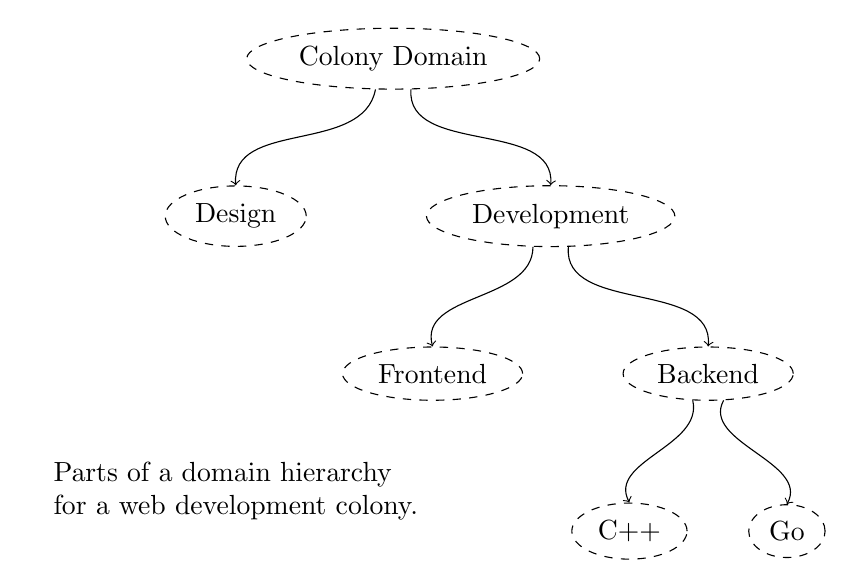
\begin{tikzpicture}
   \node[ellipse,draw, dashed] at (0,0) (tld) {Colony Domain};
   \node[ellipse,draw, dashed] at (-2,-2) (design) {Design};
   \node[ellipse,draw, dashed] at (2,-2) (development) {Development};
   \node[ellipse,draw, dashed] at (0.5,-4) (frontend) {Frontend};
   \node[ellipse,draw, dashed] at (4,-4) (backend) {Backend};
   \node[ellipse,draw, dashed] at (3,-6) (cpp) {C++};
   \node[ellipse,draw, dashed] at (5,-6) (golang) {Go}
    (tld.-120) edge[->, bend left=45, in=-120] (design.north)
    (tld.-60) edge[->, bend left=45, out=-60, in=120] (development.north)
    (development.-120) edge[->, bend left=45, in=-120] (frontend.north)
    (development.-60)  edge[->, bend left=45, out=-60, in=120] (backend.north)
    (backend.-120) edge[->, bend left=45, in=-120] (cpp.north)
    (backend.-60)  edge[->, bend left=45, out=-60, in=120] (golang.north);
  \node at (-2,-5.5) {\begin{tabular}{l} Parts of a domain hierarchy\\for a web development colony.\end{tabular}};
 \end{tikzpicture}
\end{center}

\newpage
\section{The Colonies' Own Tokens}\label{sec:colony-tokens}
Every colony has its own ERC20-compatible token. These are the tokens that, when earned as a task bounty, also create reputation for the receiver. What these tokens represent apart from this is up to the colony to establish. For example, they may have financial value, or they may be purely symbolic; some possible scenarios are outlined in Section \ref{sec:colony-token-examples}. In addition, colonies may `bring their own token' and designate an existing token as reputation-bearing.

\subsection{Managing a colony's token supply}\label{sec:colony-token-management}
In cases where a colony creates a new token, that colony is in control of changing the supply of its own tokens. More specifically, both reputation holders and token holders must agree to changes in the token supply, as both will be affected by it.

\subsubsection{Token generation and initial supply}
When a colony is created, the \ascode{TokenSupplyCeiling} and the \ascode{TokenIssuanceRate} are set. The former is the total number of colony tokens that will be created and the latter is the rate at which they become available to the colony-wide domain to assign to tasks or subdomains. The number of tokens available to the colony-wide domain can be updated at any time by a transaction from any user.

At colony creation, some tokens must also be assigned to addresses to allow users to stake tokens to create the first tasks. A one-off lump sum may also be created and made available to the colony-wide domain.

\subsubsection{Increasing the TokenSupplyCeiling}
 It is crucial that new tokens cannot be generated without widespread consensus --- especially if tokens have a financial value. Consequently, such decisions require a vote with high quorum and majority requirements involving both the token holders and reputation holders.

\subsubsection{Changing the TokenIssuanceRate}
The \ascode{TokenSupplyCeiling} represents the tokens that the token holders have granted to the colony in order to conduct business: to fund tasks and domains, and to hire workers and contributors. This is especially important during the early life of a colony when it has little-to-no revenue in other tokens to fall back on.

The \ascode{TokenIssuanceRate} controls how rapidly the colony receives the new tokens. If the rate is `too high', tokens will accumulate in the funding pot of the root domain (or other funding pots lower in the hierarchy); usually this is not a big problem. If the rate is too low, this signals that the colony has a healthy amount of activity and that the issuance rate has become a bottleneck. In such situations it may be desirable to increase the rate of issuance without necessarily increasing the maximum supply.

Increasing and decreasing the \ascode{TokenIssuanceRate} by up to 10\% can be done by the reputation holders alone and this action can be taken no more than once every 4 weeks. Larger changes to the issuance rate should additionally require the agreement of existing token holders.


\subsection{Example of token usage}\label{sec:colony-token-examples}
\subsubsection*{Tokens as early rewards}
One of the chief benefits of a colony having its own token is that it can offer rewards for work before it has any revenue or external funding to draw on.
A new colony may offer token bounties for tasks that people may accept in the hope that the reputation earned by these token payments and the future revenue earned by the colony will eventually reap financial rewards. By allowing `spending' before fund-raising, the financial burden during the start-up phase of a new colony is eased. Once a colony is profitable, payment in tokens may be the exception rather than the norm.

\subsubsection*{Tokens representing hours worked}
We could imagine a colony in which all tasks are paid in Ether, but include a number of the colony's own tokens as well, equal to the expected number of hours worked on a task. The members of the colony would be responsible for assigning `correct' token and Ether bounties to tasks. This extra responsibility would also ensure users doing the same amount of work received the same reputation gain, rather than the reputation gain being dependent on the rates they charged.

%\subsubsection*{Tokens as `fake internet points'}
%Tokens themselves need not have a monetary value; (a non-profit Colony for instance may choose to continually generate new tokens and make them available freely to anyone via a `faucet contract' in order to \emph{ensure} that they do not have a direct value). In such a situation, the token would only be valuable in a context in which payout also confers reputation.

\newpage
\section{The Reputation System}\label{sec:reputation}
\subsection{What is Reputation?}\label{subsec:what-is-reputation}

Within Colony, reputation is a number tied to an account. Reputation quantifies the contribution that user has made to the colony in recent history. Reputation will primarily be used for two things within a colony --- weighing votes of users, and determining rewards that should be allocated to users. The more reputation a user has, the more weight their vote has when making a decision. More reputation also means they receive a larger payout when rewards are issued (see Section \ref{sec:claimrewards}). We believe that because reputation is awarded to users by either direct or indirect peer approval of their actions, the consequences of this will be that influence and rewards in a colony will be assigned in meritocratic way.

\textbf{The Colony Governance System aims to be broadly meritocratic. For this reason, the majority of day-to-day decisions in a colony are weighted by the relevant reputation.} %Thus for example. any dispute in the development team will be resolved by a vote weighted by development reputation.

Unlike tokens, reputation cannot be transferred between accounts, and it cannot be bought or sold; it represents an appraisal of the account holder's activities by their peers. Reputation must therefore be earned by direct action within the colony. This reputation that is earned will eventually be lost through inaction, bad behaviour or being deemed to be wrong; an description of how reputation is gained and lost is given in Section \ref{sec:earning-losing-rep}. 

% Reputations held in one colony have no bearing on reputations held by the same account in another colony.

% Since it is not a tradable asset, reputation must be \emph{earned}. The primary method of earning reputation is by completing tasks in a colony and earning the colony's tokens. As soon as you successfully complete your first task in a colony and claim a reward of the colony's tokens, you also earn \emph{reputation} in that colony. The amount of reputation earned will be based on a combination of the performance of the user completing the task, and the payout associated with the task itself. Aside from tasks, there are administrative and managerial duties that allow users to earn reputation as well. (Section \ref{sec:earning-rep}).

% Any reputation earned is earned in a \emph{context}. The Colony Network tracks the domain in which reputation was earned and the skills associated with the action that earned it. As an example, reputation earned for the completion of a task in the `development' domain, tagged with the `solidity-dev' skill tag will be recorded as colony reputation as well as development reputation and solidity-dev reputation. (See Sections \ref{sec:rep-by-domain} and \ref{sec:rep-by-skill} for details).

% Reputation can also be lost. Any account engaged in bad behaviour will lose reputation as punishment. Furthermore \textbf{all reputation decays with time}. %Reputation has a half life of 3 months\footnote{The exact decay rate may change before release.}. 
% In order to maintain a high reputation score, an account must continue to contribute to the colony. (Section \ref{sec:losing-rep}).\\



%

%
%
\subsubsection{Reputation by Domain}\label{sec:rep-by-domain}
The organisational hierarchy of a colony provided by domains was described in Section \ref{sec:domains}. Reputation is earned in this hierarchy, and a user has a reputation in all domains that exist --- even if that reputation is zero. When a user earns or loses reputation in a domain, the reputation in all parent domains changes by the same amount. In the case of a user losing reputation, they also lose reputation in all child domains. Quantitatively, all child domains lose the same fraction of reputation that the user lost in the domain the reputation loss is notionally in. If ever a user would lose reputation and go below zero reputation, the relevant reputation becomes zero.

An example makes this clearer. Suppose a colony has a `development' domain which contains a `backend' domain and a `frontend' domain, as in Figure \ref{fig:domainhierarchysample}. Any time a member of the colony earns reputation for work completed in the backend domain, it will increase their backend reputation, their development reputation and their reputation in the all-encompassing top-level domain of the colony. Reputation earned in the development domain will only increase the development and top-level domain reputation scores of the user.

Later, the user behaves badly in the `development' domain, and they lose 100 reputation out of the 2000 they have in that domain. They also lose 100 reputation in the parent domains, and 5\% $\left(\frac{100}{2000}\right)$ of their reputation in each of the child domains of the `development' domain (which in this example, includes all of the Frontend, Backend, Node.js and Ruby domains). 

\subsubsection{Reputation by Skill}\label{sec:rep-by-skill}

We envision domains to mostly be used as an organisational hierarchy within a colony. However, this would not necessarily capture the \emph{type} of work that a user completed to earn their reputation. If the domain were a project, with tasks corresponding to both design and development work, reputation earned by completing tasks related to these skills would not be distinguishable.  To have a more fine-grained account of the type of work that a user completes to earn their reputation, the Colony Network also maintains a skill hierarchy for all colonies to use.

This global hierarchy of skills is available for all colonies to use. When a task is created, as well as being placed in a particular domain in the colony, it is also tagged with a skill from the skill hierarchy. When the worker earns reputation for successfully completing the task, they will earn reputation in the skill the task was tagged with and all parent skills. This is in addition to the reputation earned in the relevant domains. Conversely, if they are to lose reputation because their work is found inadequate, they will lose a proportional amount reputation from all child skills of the tag, if any, as is the case with the domain reputation. There is a top-level skill analogous to the top-level domain in a colony, which all skills are descendants of.

Even though the skill hierarchy is universal, reputation earned in the skill hierarchy is unique to each colony. Earning reputation in a skill in one colony has no effect on the user's reputation in that skill in any other colonies.

\subsubsection{Reputation by Colony}\label{sec:rep-by-colony}
A user's reputation in a colony is the sum of their reputation in the top-level skill and the top-level domain. This is the reputation they will be voting with in any decisions that require input from everyone in the colony. Reputation in a colony has no effect outside the colony.

\subsection{Earning and losing reputation}\label{sec:earning-losing-rep}
There are three ways to earn reputation in a colony. The first is being involved with a successfully completed task and the second is through the dispute process. In both of these cases, the user has been a productive member of the colony and is rewarded accordingly. The third way to earn reputation is upon the creation of a colony and the associated bootstrapping process (see Section \ref{sec:bootstrapping-rep}).

Reputation losses can arise from a user being found responsible for a badly executed task, or being involved in the dispute process and the dispute being resolved against them. In addition, all reputation earned by users is exposed to a continual decay over time. 

The rest of this section outlines each of these mechanisms, with references to the more detailed descriptions given elsewhere where appropriate.

\subsubsection{Reputation change from contributing to a task}\label{sec:earning-rep-from-task}
Each task requires three roles to be assigned: the administrator, the worker and the evaluator (as described in Section \ref{sec:tasks}). If the bounty for the task is denominated in the colony's token, each of these roles are eligible to earn reputation when the task is completed as long as their work was well received.

The performance of the user who has completed the work is established when the work is submitted and then evaluated. At this point, both the evaluator and the worker grade each other\footnote{These scores should be submitted using a pre-commit and reveal scheme to ensure secrecy during the rating process and avoid retaliatory grading} out of five stars.

In the case of the evaluator, a rating of 0-2 stars counts as them rejecting the work, and a score of 3-5 stars counts as accepting the work. Beyond that, we suggest the following guidelines for ratings:
\begin{itemize}
 \item[] 0 stars: user submitted no meaningful work 
 \item[]1 star:\phantom{s} user showed little activity relevant to the task, and remains far from completion on due date.
 \item[]2 stars: user was unable to complete the task, but put in a reasonable amount of effort.
 \item[]3 stars: user completed the task following the brief but there were issues during the work.
 \item[]4 stars: user completed the task acceptably and there were no complaints.
 \item[]5 stars: user completed the task to a higher standard than requested.
\end{itemize}

The actual number of reputation points $r$ earned by the worker for the completion of the task is then a function of this rating $s$ and the token payout $t$:
\begin{equation*}\label{eq:stars-to-rep}
 r = t \times \frac{2s - 5}{3}.
\end{equation*}
 
Reputation lost or gained as a function of the star rating therefore varies linearly between $-\frac{5t}{3}$ and $\frac{5t}{3}$ for zero and five stars respectively, and a rating of four stars earns the user exactly $t$. 

Similarly, the evaluator gets an amount of reputation based on their grading by the worker, but on a scale that only varies between $-t_{\rm ev}$ and $t_{\rm ev}$ (where $t_{\rm ev}$ is the evaluator's notional token payout for the task). They only earn this reputation in the current (and all parent) domains, not in the skill reputation hierarchy as they have not actually done the task. While it is likely some knowledge is required to perform the evaluation, this is not always the case; we believe that skill reputation should exclusively demonstrate ability to perform tasks.

Upon completion of a task, the administrator also earns reputation based on their token reward. There is no explicit rating of the administrator, but as with all other payments and rewards, an objection can be raised before and payout occurs. For all participants, reputation updates occur and payouts are made available only \emph{after} the objection window (described in Section \ref{sec:tasks}) has closed and all disputes  (described in Section \ref{sec:objections-and-disputes}) have been resolved at the end of the task. The reputation updates and payouts are based on the final state of the task.

\subsubsection{Reputation change as a result of Disputes}\label{sec:earning-rep-in-disputes}
If a dispute occurs, causing a vote among some portion of the colony, each side will have had to stake some number of tokens. Those who staked on the side determined to be right gain their stake back, plus some tokens that have been lost by the losing side. There will also be a reputation change as a result --- those on the losing side will lose some reputation, and some of that will be gained by the winning side. Section \ref{sec:objections-and-disputes} provides a full description of the dispute mechanism and the amount of tokens and reputation each side loses and gains.

\subsubsection{Bootstrapping reputation}\label{sec:bootstrapping-rep}
Since a colony's decision making procedure rests on reputation weighted voting, we are presented with a bootstrapping problem for new colonies. When a colony is new, no-one has yet completed any work in it and so nobody will have earned any reputation. Consequently, no objections can be raised and no disputes can be resolved as no-one is able to vote. Then, once the first task is successfully completed, that user has a dictatorship over decisions in the same domains or skills until another user earns similar types of reputation.

To prevent this, when a colony is created, the creator can choose addresses to have initial reputation assigned to them to allow the colony to bootstrap itself. There will be a global limit on the reputation that can be assigned in this manner in order to prevent an extreme reputation aristocracy. Given that reputation decays over time, this initial bootstrapping of reputation will not have an impact on the long-term operation of the colony. \textbf{This is the only time that reputation can be created without associated work being done.} Users receiving the reputation are presumably the colony creator or their acquaintances, and this starting reputation should be seen as a representation of the existing trust the creator has for their colleagues. 

We note that the same is not required when a new domain is created in a colony. We do not wish to allow the creation new reputation here, as this would devalue reputation already earned elsewhere in the colony. Happily, we can proceed without any new reputation. The colony is still able to make decisions and resolve disputes, because any objections can be escalated to a parent domain where reputation does exist, if necessary. Furthermore, even this escalation is not necessarily required in the event of a disagreement, because, even if there is no reputation in the \emph{domain} to contribute to the decision, users will still be able to vote based on their reputation in relevant \emph{skills}.

\subsubsection{Reputation Decay}
All reputation decays\footnote{The rate of decay in the final network may be different than specified here.} over time. Every 600000 blocks, a user's reputation in any domain or skill decays by a factor of 2. This decay occurs every hour, rather than being a step change every three months to ensure there are minimal incentives to earn reputation at any particular time. This frequent, network-wide update is the primary reason for the existence of the reputation mining protocol, which allows this near-continuous decay to be calculated off-chain without gas limits, and then realised on-chain. 

The decay serves multiple purposes. It ensures that reputation scores represent \emph{recent} contributions to a colony incentivising members to continually contribute to the colony. It further ensures that wild appreciations in token value (and the corresponding decrease in tokens paid per task) do not permanently distort the distribution of reputation but instead serves to smooth out the effects of such fluctuations over time.

\subsection{On-chain representation of skills and domains}\label{subsec:on-chain-representation-of-skills}
In the context of reputation, domains and skills are the same, differing only in that domains are colony-specific categorisation and skills are universal categorisation. In this subsection, each instance of `skill' should be taken to mean `skill or domain'.

Each skill that reputation can be earned in is assigned a \ascode{rep\_id} that is unique across the whole network. When a skill is created, additional properties are recorded and initialised.
\begin{equation*}
  \ascode{skill\_id} \rightarrow 
  \begin{cases}
    \ascode{n_parents} &	\textnormal{total number of parents}\\
    \ascode{parent\_n\_id} &	\parbox[t]{.6\linewidth}{\textnormal{the \ascode{rep\_id} of the $n^{\rm th}$ parent, where $n$ is an integer power of two larger than or equal to 1. }}\\
    \ascode{children}\left[\cdots\right] &	\textnormal{array of \ascode{rep\_id}s of all child skills}\\
    \ascode{n\_children} &	\textnormal{total number of child skills}
  \end{cases}
\end{equation*}
Upon creation, \ascode{children[]} and \ascode{n\_children} are empty. These two fields in all parents are updated with the \ascode{skill\_id} of the new skill on creation.\footnote{We acknowledge that this is fundamentally gas limited, but the only consequence of this will be the inability to create new skills once the maximum depth allowed by the block size is reached. Back-of-the-envelope calculations suggest this corresponds to a depth of around 80, which we don't believe our users will be limited by.}

Storing these pieces of data on-chain is required, as they are used by the reputation mining protocol (see next section) and the procedures for escalating disputes (see Section \ref{sec:objections-and-disputes}). They are stored under the control of the Colony Network contract.

\subsection{Reputation update log}\label{subsec:reputation-update-log}

Whenever an event that causes one or more users to have their reputation updated in a colony, a corresponding entry is recorded in a log in the Colony Network Contract. Each entry in the log contains

\begin{itemize}
\item The user suffering the reputation loss or gain.
\item The amount of reputation to be lost or gained.
\item The colony the update has occurred in.
\item How many reputation entries will need to be updated (including parent, child and colony-wide total reputations). This is the motivation for storing \ascode{generation} and \ascode{n\_children} for each skill and domain, as described in Section \ref{subsec:on-chain-representation-of-skills}.
\item How many total updates to reputations have occurred before this one in this cycle, including decays and updates to parents and children.
\end{itemize}

If the reputation update is the result of a dispute being resolved (as outlined in Section \ref{sec:earning-rep-in-disputes}), then instead of these first three properties, there is a reference to the dispute-specific record of stakes in the relevant colony. For the structure of this log, and an explanation of the way that it allows individual updates to be extracted in constant gas, see Appendix \ref{appendix:rep-transfer}.

This log exists to define an ordering of all reputation updates in a reputation update cycle that is accessible on-chain. In the event of a dispute during the reputation mining protocol (described in Section \ref{sec:reputationmining}), the Colony Network Contract can use this record to establish whether an update has been included correctly.


\newpage
% \section{Voting}\label{sec:voting}
Voting is a necessity in the Colony Network. In a smoothly running colony, votes will not be needed, but once there is a disagreement, or there is the need to change something that will affect a large number of people, a poll will be needed to gauge the opinion of the users of a colony.

\subsection{Reputation weighted voting}
Most votes in a colony will be due to disputes (see Section \ref{sec:disputes}). In these cases, the weights of the users' votes is proportional to the reputation that each user has in the domain and skill that the vote is taking place in. When such a vote starts, the current reputation state is stored alongside the vote. This allows the current reputation state to be `frozen' for the context of the vote, and prevents unwanted behaviours that might otherwise be encouraged (for example, delaying submission of a task until closer to voting so that the reputation earned has not decayed as much).

Voting takes place using a commit-and-reveal-scheme. To make a vote, the user submits a hash that is \ascode{keccak(secret, vote\_id)}, where \ascode{vote\_id} indicates the option that the user is voting for. Once voting has closed, the poll enters the reveal phase, where a user can submit \ascode{secret, vote\_id} and the contract calculates \ascode{keccak(secret, vote\_id)} to verify it is what they originally submitted.

As the secret is revealed it cannot be sensitive. It must also change with each vote so that observers cannot establish what people are voting for after they have revealed their first vote. We suggest a (hash) of the question the poll is asking signed with their private key. This is easily reproducible by a client at a later date with no local storage required.

When revealing their vote, the user also supplies a Merkle proof of their relevant reputation contained within the reputation state that was saved at the start of the vote. The total vote for the option they demonstrated they voted for is then incremented appropriately.

\subsection{Token weighted voting}
Unlike with reputation, we do not have the ability to `freeze' the token distribution when a vote starts. While this is effectively possible with something like the MiniMe token \cite{minime}, we envision token-weighted votes will still be regular enough within a Colony that we do not wish to burden users with the gas costs of deploying a new contract every time.

Instead, once a vote enters the reveal phase, any user who has voted on that vote will find themselves unable to see tokens sent to them, or be able to send tokens themselves --- their token balance has become locked. To unlock their token balance, they only have to reveal their vote. In this way, a user never finds themselves waiting for their tokens to unlock --- they only have to reveal the vote they cast for any polls that have entered the reveal phase. An implementation of this can be found on the Colony blog \cite{ColonyVoting}.

The primary use of a token weighted vote is related to the management of the colony tokens itself (Section \ref{sec:colony-token-management}); it seems reasonable that the decision and ability to create more tokens should lie with the colony token holders.

\subsection{Hybrid voting}
A hybrid vote would allow both reputation holders and token holders to vote on a decision. When such a vote takes place, the total reputation and the total token holdings each represent 50\% of the voting weight.

% \newpage

\section{Calculating Reputation: Miners and Merkle Proofs}\label{sec:reputationmining}
The reputation system is a core component of any decentralised colony. By carefully balancing the rewards and penalties we aim to keep every users' incentives aligned with the colony and the colony network. Since reputation can only be \emph{earned} and not transferred between accounts, the system fosters a more meritocratic form of decision making than pure token-weighted voting can hope to achieve. The continuous decay of reputation ensures that the influence conveyed by reputation is recently earned and up-to-date. As such, it prevents a reputation aristocracy and allows for a fluid passing of control from one set of contributors to another over time.


Due to the combined complexity of reputation scores across multiple colonies, domains, and skills, reputation scores cannot be stored or calculated on-chain. Instead, the calculations will all take place off-chain, the results of which will be reported to the blockchain by participating CLNY holders --- in a process resembling a proof-of-stake blockchain consensus protocol. We call this procedure \textbf{`Reputation Mining'}.

The reputation calculation whose result the miners are submitting is determined by the activities that have taken place in the colonies and can be fully deterministically derived from the ethereum blockchain. Game-theoretically the system is protected similarly to the off-chain calculations of TrueBit (\cite{TruebitWhitepaper}) in that, \emph{while the calculation cannot be done on-chain and a correct submission can never be proved true, an incorrect calculation can always be proved to be wrong}.


\subsection{Merkle Trees and Proofs}\label{sec:Merkle-summary}
This subsection contains only a summary of Merkle trees (\cite{MerkleTrees}, \cite{MerkleInEthereum}) and Merkle proofs in order to establish some terminology, and can be skipped if already familiar with them.

Consider the tree shown in Figure \ref{fig:Merkleexample}. The data leaves of the tree (1, 2, 3 and 4) are each hashed individually to give A, B, C and D. These are then repeatedly hashed pairwise until only a single hash remains, indicated by G in Figure \ref{fig:Merkleexample}. In the event of a starting or an intermediate array being an odd number (which will always happen for a starting array that is not a power of two), the hash contained in the last element is hashed with itself.

The resulting structure is known as a Merkle tree. In order to prove that the element \ascode{1} is in the tree with root \ascode{G}, one submits a Merkle proof containing the information \ascode{1, [B,F], [l,l]}. The first argument is the element whose existence is to be proved. The second argument is the list of hashes that the hash of the first element should be hashed with in succession. The last argument is an array of \ascode{l}'s and \ascode{r}'s that indicates whether the hash calculated so far should be hashed on the left or the right of next element in question. So to show that \ascode{3} was in the tree with root \ascode{G}, the proof would be of the form \ascode{3, [D,E], [l,r]}.
\begin{figure}
\centering
 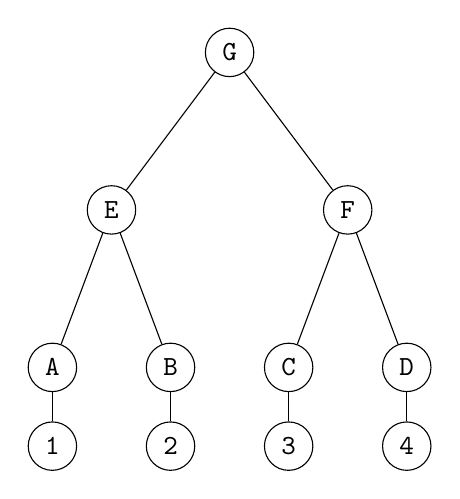
\begin{tikzpicture}
  \node[shape=circle, draw] at (0,-4) (a) {\texttt{A}};
  \node[shape=circle, draw] at (0,-5) (1) {\texttt{1}}
   edge[-] (a);
  \node[shape=circle, draw] at (1.5,-4) (b) {\texttt{B}};
  \node[shape=circle, draw] at (1.5,-5) (2) {\texttt{2}}
   edge[-] (b);

  \node[shape=circle, draw] at (3,-4) (c) {\texttt{C}};
  \node[shape=circle, draw] at (3,-5) (3) {\texttt{3}}
   edge[-] (c);
  \node[shape=circle, draw] at (4.5,-4) (d) {\texttt{D}};
  \node[shape=circle, draw] at (4.5,-5) (4) {\texttt{4}}
   edge[-] (d);
  %
  \node[shape=circle, draw] at (0.75,-2) (e) {\texttt{E}}
   edge[-] (a)
   edge[-] (b);
  \node[shape=circle, draw] at (3.75,-2) (f) {\texttt{F}}
   edge[-] (c)
   edge[-] (d);
  %
  \node[shape=circle, draw] at (2.25,0) (g) {\texttt{G}}
   edge[-] (e)
   edge[-] (f);
 \end{tikzpicture}
 \caption{A simple Merkle tree. Elements A, B, C and D correspond to the hashes of 1, 2, 3 and 4. E is the hash of A concatenated with B.}
 \label{fig:Merkleexample}
\end{figure}

Note also that the array of \ascode{l}'s and \ascode{r}'s nothing more than a binary representation of the leaf node's index in the tree. When expressed in this way, we refer to the index as the `path' in the Merkle proof. We refer to the objects that get hashed along the way (i.e. \ascode{D} and \ascode{E}) as the `siblings'.


\subsection{The Reputation Tree and the ReputationRootHash}\label{sec:reptree}
The data leaves in the reputation tree are the reputations all users have in all skills, as well as the colony-wide totals. Such a leaf consists of the following data:
\[
R =
\begin{cases}
 \ascode{rep\_id} & \textnormal{the id of a skill or domain identifying the type of reputation},\\
 \ascode{colony\_id} & \textnormal{the colony the reputation is held in},\\
 \ascode{user} & \textnormal{the address holding the skill},\\
 \ascode{amount} & \textnormal{the numerical value of the reputation}.
\end{cases}
\]

All individual reputations are assembled into the \textbf{``Reputation Tree''} which is a Merkle tree of all individual reputations in a colony, as well as the total reputation of each type held by the users in each colony. The leaves that represent these colony-wide totals are indicated by setting \ascode{user} to zero. These leaves are then put into a Merkle tree in the usual way (described in Section \ref{sec:Merkle-summary}).\footnote{The ordering of the data leaves is only determined by when these reputations were first earned.} We term the root hash of the resulting tree the \ascode{ReputationRootHash}, $\mathcal{RH}$.
\begin{figure}
\centering
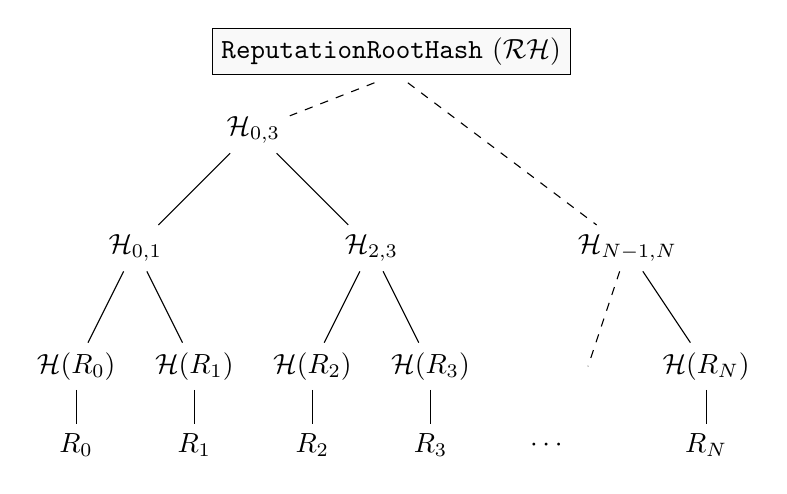
\begin{tikzpicture}
 \node at (0,-5) (r0) {$R_0$};
 \node at (1.5,-5) (r1) {$R_1$};
 \node at (3,-5) (r2) {$R_2$};
 \node at (4.5,-5) (r3) {$R_3$};
 \node at (6,-5) (rdots) {$\cdots$};
 \node at (8,-5) (rn) {$R_N$};
 %
 \node at (0,-4) (r0hash) {$\mathcal{H}(R_0)$}
  edge[-] (r0);
 \node at (1.5,-4) (r1hash) {$\mathcal{H}(R_1)$}
  edge[-] (r1);
 \node at (3,-4) (r2hash) {$\mathcal{H}(R_2)$}
  edge[-] (r2);
 \node at (4.5,-4) (r3hash) {$\mathcal{H}(R_3)$}
  edge[-] (r3);
 \node at (8,-4) (rnhash) {$\mathcal{H}(R_N)$}
  edge[-] (rn);
 %
 \node at (0.75,-2.5) (r01) {$\mathcal{H}_{0,1}$}
  edge[-] (r0hash)
  edge[-] (r1hash);
 \node at (3.75,-2.5) (r23) {$\mathcal{H}_{2,3}$}
  edge[-] (r2hash)
  edge[-] (r3hash);
 \node at (7,-2.5) (rnn) {$\mathcal{H}_{N-1,N}$}
  edge[-] (rnhash)
  edge[dashed] (6.5,-4);
 %
 \node at (2.25,-1) (r14) {$\mathcal{H}_{0,3}$}
  edge[-] (r01)
  edge[-] (r23);
 %
 \node[draw, fill=gray!5] at (4,0) (root) {\texttt{ReputationRootHash}  ($\mathcal{RH}$)};
 \node[below = 1mm of root] (dummy) {\phantom{a}}
  (dummy.north west) edge[dashed] (r14)
  (dummy.north east) edge[dashed] (rnn);
 %
 %
\end{tikzpicture}
\caption{The Merkle tree of users' reputations with \ascode{ReputationRootHash} as the root. We use $\mathcal{H}$ to indicate the \ascode{keccak256} hash function. Above the second row, each element is the hash of the concatenation of its two children.}
\end{figure}


The \ascode{ReputationRootHash} is the only data we record on the blockchain associated with users' reputations. It summarises the state of the whole reputation system and whenever a user wishes to make use of their reputation, they can submit a Merkle proof from the reputation $\mathcal{R}_i$ they wish to make use of and ending at $\mathcal{RH}$.

\subsection{Calculating the new root hash}
To calculate the new root hash, the miners begin with the last reputation state, and decay all reputations held by all users in all colonies, in the order of the leaves in the tree. They then take the set of reputation gains or losses that were not in the last state submitted, and are to be included in the next state. They apply the reputation updates to each user in each colony, updating or adding leaves as necessary, to end up with a new list of reputations for all users and colonies. These new reputations are then hashed and assembled into a new Merkle tree yielding an updated \ascode{ReputationRootHash}.

While the calculation is too large to be done on-chain due to technical and economic limitations (i.e. the block gas limit and the cost of gas, respectively), this calculation can easily be performed by a typical user's computer.

\subsection{Submission of a new root hash}
%
\subsubsection*{What is submitted?}
The final \ascode{ReputationRootHash} is submitted to the contract by the miner along with the number of leaves in the tree. Further, the miner also submits the IPFS or Swarm hash of a document containing the entire state tree, though this is only for convenience; any user can construct this locally based on the blockchain history.
%
\subsubsection*{Who can submit a new root hash?}
All CLNY token holders are eligible to become miners and participate in the reputation update process, but since any user can calculate the correct root hash locally, it would be possible for \emph{any} miner to submit the hash to the contract.

It is however undesirable to have too many submissions for every update. We propose a mechanism that only allows some miners to submit results to begin with. To participate in the mining process, \rcths\ must stake some of their tokens to become `reputation miners'. A submission will only be accepted from a miner if
\begin{equation*}\label{eq:mining-difficulty}
\ascode{keccak256(address, N, hash)} < \ascode{target}.
\end{equation*}
At the beginning of the submission window, the target is set to 0 and slowly increases to $2^{256}-1$ after 150 blocks. We limit the total number of miners allowed to submit a specific hash to 12.

The variable $N$ that goes into the hash is some integer greater than 0 and less than the number of tokens the \rcth\ address has staked divided by $10^{15}$, meaning that users with a large stake have a higher chance of qualifying to submit a hash sooner than smaller stake holders. The factor of $10^{15}$ is introduced to ensure that all hashes a user is eligible to submit can be calculated in a few seconds by the client. It also effectively creates a minimum number of tokens that must be staked to submit a hash. This puts a tangible cost on any attacks revolving around spamming known false submissions (see Section \ref{sec:mining-possible-attacks}).

Miners will also be required to have staked their tokens for a few update cycles before they are eligible to submit or support a hash.
%
\subsubsection*{Verifying a submission}
If only one state is submitted by the end of the submission period, then the new state is accepted, and proposals of the next state can begin to be made. This is expected to be the most common occurrence.

If more than one state has been submitted, then either someone has made a mistake, or there is a malicious entity trying to introduce a fraudulent reputation change. In this event, the a challenge-response protocol can establish which state is incorrect (see Section \ref{sec:challengeresponse})

\subsubsection*{Mining Rewards}

When a state is accepted, a number of (newly minted) \rcts\ are made available for the users who submitted the correct state to claim as a reward. They also receive a corresponding amount of reputation in the \rc\ (in a special mining skill, which only users in the \rc\ can earn by performing this task). This reputation update is no different from any other, aside from the limitations of who is able to earn it, and will be included in the subsequent reputation update cycle. The size of the rewards and their distribution are described in Section \ref{subsec:mining-costs-and-rewards}.

\subsection{Dealing with false submissions}\label{sec:challengeresponse}
%
\subsubsection{The Challenge-Response Protocol}

We assume that the correct hash is one of the  submitted hashes. This is a reasonable assumption, as only one out of all the miners is required to make a correct submission, and there is an incentive for them to do so (the reward defined in Section \ref{subsec:mining-costs-and-rewards}). Thus our task is not to validate the correct hash but to invalidate the false ones.

We must prove all but one submission incorrect by having each submission navigate a series of \emph{challenges}. These challenges refer to events that happened in the colony network within the last update cycle that have an effect on reputation. The \emph{responses} to the challenges are Merkle proofs that the corresponding reputation update was properly handled. Anyone is able to respond to a challenge, regardless of who submitted the original hash; this should ensure that the correct state is always defended.

We begin with the scenario where only two submissions are made, and one is correct.

First we consider the case in which the same hash has been submitted twice, but with a disagreement about the number of leaves it contained. In this situation, the users are required to submit a Merkle proof for the last leaf in their tree. We are able to tell if a submitted proof corresponds to the last leaf in the tree, as all sibling hashes must be hashed on the left. Noting the positions in the Merkle proof in which a hash is hashed with itself also allows us to tell the index of this last leaf; if it corresponds to either of the submitted states, that one is correct.

We now consider the more complicated case where two different hashes have been submitted.

\subsubsection*{1. The Justification Tree}
  \newcommand{\jrh}{\ensuremath{\mathbb{JRH}}}
The first step is for both parties to upload a justification of their submitted hash. This justification consists of a second Merkle root and two Merkle proofs.

The Merkle root in questions is the \ascode{JustificationRootHash} (\jrh); it is the root of the `Justification Tree' -- a tree where each leaf represents a complete reputation state i.e. each leaf is a \ascode{ReputationRootHash}.

The left-most leaf of the Justification Tree ($\mathcal{RH}_0$) is the final accepted reputation state from the last update. Both parties must submit a proof that their tree does indeed start at $\mathcal{RH}_0$. Note that in a Merkle proof for a left-most leaf, all siblings are hashed on the right.

The right-most leaf of the Justification Tree ($\mathcal{RH}_n$) is the \ascode{ReputationRootHash} they originally submitted. Both parties must submit a Merkle proof that their tree does indeed end with this hash. Note that in a Merkle proof for a right-most leaf, all siblings are hashes on the left; furthermore, by noting the steps at which a hash is hashed with itself, we can determine the index of the last leaf. This index is required to be $n$ --- the number of reputation updates in the log.

The intermediate leaves of the Justification Tree represent the evolution of the reputation state, with $\mathcal{RH}_i$ corresponding to the reputation state after the first $i$ reputation updates in this cycle have been applied.

 %
\begin{figure}
\centering
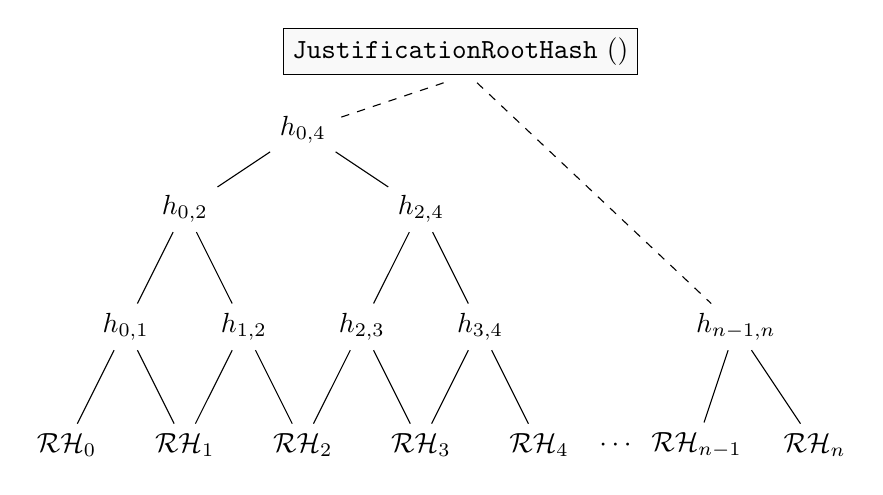
\begin{tikzpicture}
 \node at (0,-4) (rh0) {$\mathcal{RH}_0$};
 \node at (1.5,-4) (rh1) {$\mathcal{RH}_1$};
 \node at (3,-4) (rh2) {$\mathcal{RH}_2$};
 \node at (4.5,-4) (rh3) {$\mathcal{RH}_3$};
 \node at (6,-4) (rh4) {$\mathcal{RH}_4$};
 \node at (7,-4) (rdots) {$\cdots$};
 \node at (8,-4) (rhn1) {$\mathcal{RH}_{n-1}$};
 \node at (9.5,-4) (rhn) {$\mathcal{RH}_n$};
 %
 \node at (0.75,-2.5) (rh01) {$h_{0,1}$}
  edge[-] (rh0)
  edge[-] (rh1);
 %
 \node at (2.25,-2.5) (rh12) {$h_{1,2}$}
  edge[-] (rh1)
  edge[-] (rh2);
 %
 \node at (3.75,-2.5) (rh23) {$h_{2,3}$}
  edge[-] (rh2)
  edge[-] (rh3);
 %
 \node at (5.25,-2.5) (rh34) {$h_{3,4}$}
  edge[-] (rh3)
  edge[-] (rh4);
 %
 \node at (8.5,-2.5) (rhnn) {$h_{n-1,n}$}
  edge[-] (rhn)
  edge[-] (rhn1);
 %
 \node at (1.5,-1) (rh02) {$h_{0,2}$}
  edge[-] (rh01)
  edge[-] (rh12);
 %
 \node at (4.5,-1) (rh24) {$h_{2,4}$}
  edge[-] (rh23)
  edge[-] (rh34);
 %
 \node at (3,0) (dummy14) {$h_{0,4}$}
  edge[] (rh02)
  edge[] (rh24);
 %
 \node[draw, fill=gray!5] at (5,1) (root) {\texttt{JustificationRootHash} (\jrh)};
 \node[below = 1mm of root] (dummy) {\phantom{a}}
  (dummy.north west) edge[dashed] (dummy14)
  (dummy.north east) edge[dashed] (rhnn);
 %
 %
\end{tikzpicture}
\caption{The Justification Tree. Note that each intermediate leaf $\mathcal{RH}_i$ is hashed into the tree twice. }
\label{fig:justification-tree}
\end{figure}
An example of such a tree is shown in Figure \ref{fig:justification-tree}. Note that in the first stage of the tree, every neighbouring pair of data leaves is hashed, and so any pair has a shared Merkle proof to the root. We do this so that each element in the first row of hashes (indicated by $h_{0,1}, h_{0,2} \ldots h_{n-1,n}$ in Figure \ref{fig:justification-tree}) represents a transition between two states. It is these transitions that are the subject of the mining dispute resolution process.

Since any two differing submitted states agree on the first leaf $\mathcal{RH}_0$ (which is the \ascode{ReputationRootHash} accepted at the end of the previous iteration of the mining process), and disagree on the last leaf $\mathcal{RH}_n$ (the hash they submitted), there must be a hash ($h_{i,i+1}$) that represents the transition from $\mathcal{RH}_i$ to $\mathcal{RH}_{i+1}$) where they agree on the starting state but disagree on the result. This transition is meant to be the effect of a single reputation update (the $i^{th}$)\footnote{We start counting at zero, i.e. the transition from $\mathcal{RH}_{0}$ to $\mathcal{RH}_{1}$ is the `zeroth'.}, and this is the reputation update we will calculate on-chain to establish which submission is incorrect.\\

\noindent First, however, we must establish where the two submissions first differ.

\subsubsection*{2. Searching for the discrepancy}
The contract requires both parties to submit repeated Merkle proofs that specific reputation updates were handled correctly until the first discrepancy between the two submissions is found.

We shall call the two parties $A$ and $B$ and we shall indicate which party made a submission by a superscript of $A$ or $B$. Furthermore we introduce the simplifying notation of $\overline{h}$ to mean `sibling of $h$' in the Merkle tree. Recall that if $h$ does not have an immediate sibling, $\overline{h}$ is taken to be equal to $h$ as per our rule of hashing these elements with themselves.

Along with their justification root hashes $\jrh^A$ and $\jrh^B$ both parties have already submitted proofs for the left-most leaf. These proofs have the simplified\footnote{Since we know that the proofs concern the first and last leaf of the tree, no array of left-right information is needed.} form:
\[
 \overline{\mathcal{RH}_0}^A, \overline{h_{0,1}}^A, \overline{h_{0,2}}^A, \ldots \overline{h_{0,2^k}}^A \qquad \textnormal{ terminating at } \jrh^A
\]
and
\[
 \overline{\mathcal{RH}_0}^B, \overline{h_{0,1}}^B, \overline{h_{0,2}}^B, \ldots \overline{h_{0,2^k}}^B \qquad \textnormal{ terminating at } \jrh^B
\]
where $k$ is the largest integer such that $2^k$ is smaller than $n$.

When the first miner (say $A$) submits their proof the contract saves the values of $h_{0,2^k}^A$ and $\overline{h_{0,2^k}}^A$. When the second miner submits their proof the contract compares $h_{0,2^k}^A$ to $h_{0,2^k}^B$. If they are not equal, the contract saves both of these values (and forgets $\overline{h_{0,2^k}}^A$). If they are equal, the contract retains the values of $\overline{h_{0,2^k}}^A$ and $\overline{h_{0,2^k}}^B$ (forgetting $h_{0,2^k}^A$).

The rationale behind this behaviour is the following: If $h_{0,2^k}^A = h_{0,2^k}^B$ then the two justification trees are equal between $\mathcal{RH}_0$ and $\mathcal{RH}_{2^{k-1}}$ and the first discrepancy must lie in the right-hand subtree whose root is $\overline{h_{0,2^k}}^A$ for miner $A$ and $\overline{h_{0,2^k}}^B$ for miner $B$. If on the other hand $h_{0,2^k}^A \neq h_{0,2^k}^B$, then the first discrepancy must lie in the left-hand subtrees given by $h_{0,2^k}^A$ and $h_{0,2^k}^B$. The situation is summarised by
\begin{eqnarray*}
 h_{0,2^k}^A \neq h_{0,2^k}^B & \Longrightarrow & \textnormal{First discrepancy occurs at some } \mathcal{RH}_i \textnormal{ with } 0 \leqslant i < 2^k\\
 h_{0,2^k}^A = h_{0,2^k}^B & \Longrightarrow & \textnormal{First discrepancy occurs at some } \mathcal{RH}_i \textnormal{ with } 2^k \leqslant i < n
\end{eqnarray*}

The contract begins its search by %pseudorandomly%\footnote{This pseudorandomness is to help mitigate an attack described in Section \ref{sec:mining-possible-attacks}.}
%picking an index $j$ from within the range the first discrepancy in known to lie in. It then
%
picking an index $j$ from within the range the first discrepancy in known to lie in (say always the smallest), and requiring both parties to provide a Merkle proof showing how the $j^{th}$ reputation update from all updates to be applied this cycle (Section \ref{subsec:reputation-update-log}) was included in their justification tree. The required target of this proof is no longer the $\jrh$ itself, but rather the retained value for $h_{0,2^k}$ or $\overline{h_{0,2^k}}$. Specifically this proof consists of

\begin{itemize}
 \item[(i)] The root hash before the update was applied ($\mathcal{RH}_{j}$).
 \item[(ii)] The root hash after the update was applied ($\mathcal{RH}_{j+1}$).
 \item[(iii)] A Merkle proof showing the inclusion of $h_{j,j+1}$ in the relevant justification sub-tree.
\end{itemize}

The same process as before of comparing hashes and retaining the roots of either the left-side subtree or the right-side subtree is repeated. With each iteration, the range of possible values for the index of the first discrepancy is reduced by (on average) a factor of two and the length of the required Merkle proofs is reduced by one.

% and requires both parties to provide:
% \begin{itemize}
%  \item[(i)] The root hash before the update was applied ($\mathcal{RH}_{i-1}$).
%  \item[(ii)] The root hash after the update was applied ($\mathcal{RH}_i$).
%  \item[(iii)] A Merkle proof showing that the pair ($\mathcal{RH}_{i-1}, \mathcal{RH}_i$) is correctly included in the justification tree.
% \end{itemize}
%
% When either party submits, first their Merkle proof is checked. It must use the correct sequence of \ascode{l} and \ascode{r} during the hashing process, which is defined by the $i$ that has been selected. If the Merkle proof is correct, then if this is the first party to submit, their $\mathcal{RH}^A_{i-1}$ and $\mathcal{RH}^A_{i}$ are stored. We label these with a superscript `A' to denote they have come from the first party to submit.
%
% When the second party submits and their Merkle proof is found valid, then the contract compares the submitted $\mathcal{RH}^B_{i-1}$ and $\mathcal{RH}^B_{i}$ to $\mathcal{RH}^A_{i-1}$ and $\mathcal{RH}^A_{i}$ stored from the first party's submission.
%
% If the pairs of submitted root hashes are identical, the (first) discrepancy between the two calculations occurs must occur later in the tree. The lower bound for the search for the first discrepancy can be set to $i+1$. If the submitted root root hashes are such that $\mathcal{RH}^A_{i-1}\neq\mathcal{RH}^B_{i-1}$ and $\mathcal{RH}^A_{i}\neq\mathcal{RH}^B_{i}$, then the first discrepancy must occur later in the tree. The upper bound for the search can be set to $i-2$.
%
% This process repeats, pseudorandomly selecting a new $i$ within the still-valid bounds of the search for the new challenge. Each newly submitted proof further reduces the size of the search space by a factor of two on average.\footnote{By examining precisely at which sibling the first discrepancy occurs, some stages of the binary search could be skipped. However, in order to accomplish this all the siblings of the proof that first completed the challenge would need to be stored on the blockchain, so it is more gas efficient to do the na\"{i}ve binary search for all but the very smallest of trees.}

There are two ways this process can terminate. The first way the process terminates is when one party does not respond to a challenge. In this case the party not responding is deemed to be incorrect.

The other way the process terminates, is when it has reached the bottom of the tree and found $h_{i-1,i}^A = h_{i-1,i}^B$ while $h_{i,i+1}^A \neq h_{i,i+1}^B$. The process has thus determined that it is the $i^{th}$ reputation update from the log where the two submissions differ (i.e. they agree on $\mathcal{RH}_{i}$ but not on $\mathcal{RH}_{i+1}$).

Once the contract has found the index $i$ such that $\mathcal{RH}^A_{i}=\mathcal{RH}^B_{i}$ but $\mathcal{RH}^A_{i+1}\neq\mathcal{RH}^B_{i+1}$, the contract then requires each party to submit
\begin{itemize}
 \item[(iv)] A Merkle proof for the reputation ($R_j$) affected by the $i^{th}$ update transaction.
\end{itemize}

The Merkle proof that proves the inclusion of $R_j$ (before the reputation update) in the reputation root hash $\mathcal{RH}_{i}$ and the Merkle proof of the inclusion of $R_j$ (after the reputation update) in $\mathcal{RH}_{i+1}$ must only differ in the state of the reputation $R_j$ itself. This is because the reputation trees with roots $\mathcal{RH}_{i}$ and $\mathcal{RH}_{i+1}$ differ in only a single leaf (that of $R_j$).\footnote{In the case of the addition of a new leaf, the proof for an $R_j$ before the update is replaced by a proof for the current last leaf in the tree. They also submit the merkle proof for the new $R_j$ after the update. These two proofs submitted will differ in more than just $R_j$, but if valid must converge at a predictable location in the Merkle proof, dependant on the number of leaves in the tree. }

When either party submits valid Merkle proofs, showing that the before and after state they claim to be correct is included in the $\mathcal{RH}_{i}$ and $\mathcal{RH}_{i+1}$ in their justification tree, the reputation update is also calculated on-chain to determine whether the submitting party has done their calculation correctly. If the calculation was not done correctly, the submission is identified as false.

The process does not terminate until \emph{both} parties have submitted their proofs, or the timeout is reached. There is an edge case in which it appears as if the first to submit has done the calculation correctly, but in actual fact has erroneously added a new leaf in the reputation tree (see Section \ref{sec:earning-rep-for-first-time}) even though no new leaf was required. This error can be identified when the other party submits a correct proof.

If there are more than two submissions for the new \ascode{ReputationRootHash}, this process is conducted in parallel between multiple pairs of submitted hashes, and then repeated, until only one submission remains.

If less than an hour elapses from submissions opening to only one submission remaining, the next submission window only opens when an hour has passed from the start of this window. If more than an hour has passed, the next submission window opens immediately.

\subsubsection*{Gas-cost Considerations and Alternative Implementations}
There is a trade-off between the number of transactions needed until the first discrepancy between two submissions is found and the size of the storage required by the contract. As written above, the contract stores only the last hashes of the Merkle proof, thereby reducing the range of possible values of $i$ by a factor of two at each step. If the contract stores more of the submitted hashes that constitute the Merkle proofs, the range can be reduced faster and fewer challenges will be required. Ultimately it will be a gas-cost analysis that determines the exact algorithm to use.

We also note at this point that a malicious submission, performing the attack described in Section \ref{sec:mining-possible-attacks}, can carefully craft their false justification trees to require the maximum number of challenges to resolve. Such a worst-case submission can not be made in the alternative implementation in which the full\footnote{Or as much of the head and tail of the Merkle proofs as the gas limits will allow.} Merkle proofs are stored (and compared) on-chain, and in which challenges are issued for an index $j$ picked pseudorandomly from within the range of possible values.

\subsection{Calculating reputation updates}\label{sec:calculating-reputation-updates}
%
\subsubsection{Keeping track of reputation changes}
%
Fundamentally, there are two types of reputation update that occur:
\begin{itemize}
 \item Decay of existing reputation.
 \item Addition or removal of reputation as a reward or punishment.
\end{itemize}

When a user earns reputation in a skill or domain, they also earn reputation in all parent domains, which corresponds to $2\times\left(\ascode{n\_parents}+1\right)$ reputation updates. Alternately, when a user loses reputation, they also lose reputation in all parents and all children representing a total number of updates of $2\times\left(\ascode{n\_parents} + \ascode{n\_children} + 1\right)$. The factors of two here come from also updating the relevant colony-wide totals.

In Section \ref{subsec:on-chain-representation-of-skills}, we asserted we store \ascode{n\_parents} and \ascode{n\_children} for all skills and domains. It is only by having access to the number of parents and children for each reputation and the reputation update log recording how many reputations have been updated already in this update cycle (via \ascode{n\_updates}) that the resolution protocol is able to perform the binary search of the justification trees submitted by the disagreeing users. At the start of the challenge protocol, the contract can look up the last entry in the update table for the cycle under consideration, and work out how many updates have occurred in this cycle based on the number of updates prior and the number of parent and child reputations. After verifying that both submitted justification trees contain this exact number of leaves it can proceed to the binary search.

When the discrepant state transition is found, the users supply the index of the event in the on-chain log that corresponds to that reputation update.  This means that the contract does not have to iterate over the whole list expensively, but the contract can simply check the correct reputation update is being considered, and then confirm that the calculation made corresponds to the correct reputation update. To do this, we assert that children are always updated in order, then parents, and then the reputation in question itself. In addition, all colony-wide totals of reputation are always updated in this order before any user-specific reputation.

If the discrepant transition is a decay transition they must also supply a Merkle proof that the starting value assumed for the user corresponds to the value that user had at the end of the last update cycle. A decay transition is identified by the Merkle path corresponding to an index in the justification tree smaller than the number of leaves in the reputation tree at the end of the last successful update.

Recording the number of leaves in the reputation tree is required % to allow the binary search to occur, as well as
to accommodate the decay calculations that must be done at the start of each update. Before any new reputation is earned or lost in an update cycle, all existing reputations owned by users decay (see Section \ref{sec:repdecay}). There is a decay calculation for every leaf in the previously accepted reputation tree. We do the decay calculations first to give users the benefit of the doubt during reputation updates so they do not lose reputation they have only just earned to premature decay.

\subsubsection{Earning reputation for the first time}\label{sec:earning-rep-for-first-time}
When a user earns reputation in a new skill, at least one new leaf is added to the tree --- if they have not earned reputation before in some of the parents, then they will also cause further new leaves to be added. Additional new leaves will be added if they are the first user in a colony to earn those particular skills, making the total reputation for that skill in the colony non-zero. During a dispute, when the user proves that they have included the update in the tree, it is not possible to check (efficiently) on-chain that they should not have added it to an existing leaf instead. However, because during the resolution process we are always comparing two submissions against each other, one of two things will be true:\footnote{Assuming that one of the two submissions is correct.}
\begin{itemize}
 \item Both submissions added a new leaf to the tree. If there was a discrepancy, then it is in the maths conducted on this leaf, not the addition of the leaf itself. The maths can be checked on-chain to establish which result is correct.
 \item One submission adds the new reputation to an existing leaf (the correctness of which can be checked on-chain easily). In this case, the user who added the leaf incorrectly is wrong.
\end{itemize}

\subsubsection{Transfers of reputation between accounts}\label{sec:reptransfer}

The most important quality of reputation that distinguishes it from a token is that it is tied to an account and cannot be transferred. However, in the event of disputes (Section \ref{sec:objections-and-disputes}) it can happen that one party to a dispute loses reputation while the other gains. This process has to be modelled as a `reputation transfer' to ensure that reputation is never created in this process (i.e. the reputation lost by the loser is at least as much as the reputation gained by the winner).

If an entry in the reputation update log indicates that a dispute has occurred and been resolved, then there will be a number of transfers of reputation between users represented by a single entry. Each such transfer will have to accommodate the updates of all the parents of the reputation being gained by one user, and updates of all the parents and children of the reputation being lost by the other. However, we have to ensure that the user who is losing reputation still has the reputation to lose if another user is gaining it.

To achieve this, all the transactions that correspond to updating the reputations of the user gaining the reputation are done first. In the event such a transaction must be proved to be correct in the resolution protocol, the users can provide a proof of the losing user's reputation, prior to them losing it in this event in update cycle, and this can be compared to the amount of reputation intended to be gained. Whichever is smaller is used as the amount of reputation the user is gaining during the calculations.

Then, when calculating the reputation deduction to be applied to the losing user, the reputation that was used as the voting weight should be done last i.e. all the children and parents should be considered first, as it is the amount of the reputation that was eligible to vote that will determine the fraction lost of each of the child reputations. %If any of these calculations need to be proved correct during the resolution protocol,

For further details about reputation transfers and disputes, see Appendix \ref{appendix:rep-transfer}.

\subsubsection{The Reputation Decay Calculation}\label{sec:repdecay}
The reputation decay process was described above as being continuous. In practise, it will decay by a small, discrete amount during each reputation update cycle following an exponential decay. However, such a calculation is not possible to do accurately on-chain during the resolution protocol, so we must use an approximation. The details of the approximation we use, and a proof that this approximation is accurate and will not affect the running of (active) colonies can be found in Appendix \ref{appendix:rep-decay}.

\subsection{Denial of service attacks}\label{sec:mining-possible-attacks}

In the event of multiple submissions, finding the correct one takes time --- the timeout $t$ for the challenge-response must be reasonable to allow the transaction defending a submission to propagate and be mined. A denial-of-service attack is therefore possible, whereby an attacker makes many false submissions. However, if these false submissions were random hashes, unable to be defended, then none would be defended correctly within the first timeout window, and the attack would quickly end. For pairings where neither submission is defended, any user can remove both submissions from consideration and claim the tokens that were staked to allow submission.

The denial of service attack (to delay a proper reputation update) can only be sustained when the false submissions are incorrect only in some leaves, and the majority of the justification tree is correct. In this scenario, the attacker successfully defends each of their submissions for as long as possible to delay the resolution of the reputation mining protocol as much as possible.

Any such attack is capped by the first round of pairings of submissions against each other. Even if the attacker made millions of submissions, only a finite number of those would be able to be successfully defended due to the block size --- currently, no more than 4500 submissions would be able to be defended, even if the attacker used up all block space during the timeout.\footnote{These figures assume $1.5\pi\times10^6$ gas in a block, and that each transaction is only 21000 gas for a worst-case-scenario calculation.} With only 4500 submissions able to make it to the second round, the length of time the DoS attack would be sustained for is given by

$$t \times \left\lceil\log_2\left(4500\right)\right\rceil\times \left\lceil\log_2\left(N_{\rm updates}\right)\right\rceil$$

\noindent where $N_{\rm updates}$ is the number of reputation updates that have been made in this update cycle. To arrive at this figure, we know there will need to be $\left\lceil\log_2\left(4500\right)\right\rceil$ rounds of comparison between submissions to eliminate all but one. Each round will require $\left\lceil\log_2\left(N_{\rm updates}\right)\right\rceil$ interrogations of the justification tree to establish where the two submissions being compared differ. Finally, each interrogation can take up to $t$ before it is considered to have timed out and one or both of the submissions is deemed invalid. The product of these three factors tells us how long this reputation update can be delayed by an attacker.

Long term, $N_{\rm updates}$ will be dominated by the decay transactions rather than by any updates that have occurred since the last reputation state was established. Even if the Colony Network were wildly successful, with 100000 colonies, each with 1000 users that had earned some reputation in 1000 different skills in each of the structural and skill hierarchies, and using 5 minutes as the value of $t$, the delay to the reputation updates would only be around $36$ hours. Recent congestion on the ethereum network has shown that we will need to be able to accommodate situations where block space is at a premium; the reputation mining client will need to recognise when this is occurring, and send transactions with higher gas prices as appropriate in order to meet the timeout deadline.

There would be little effect on the rest of the Colony Network in this time. Users would still be able to exercise their reputation from the previous reputation update, and continue to influence decisions with that reputation. Indeed, this shows what perhaps the main motivation for such an attack would be --- if a user knew that they had been `caught' behaving badly, and was due to lose all their reputation, they might try such an attack to eke out the last bits of influence they possibly could. However, decisions in the Colony network do not resolve quickly, and in a well-developed colony we would not expect any one person to have a large amount of reputation when compared to the rest of the colony. It therefore seems unlikely any one user would be able to unduly influence decisions significantly while conducting such an attack.

Assuming this attack continued, then the reputation mining protocol would effectively only update every 36 hours. Users staking would become more susceptible to variance in terms of the rewards, but otherwise little would change in the day-to-day functioning of any individual colony.

However, the attacker would lose \emph{all} the \rct\ that they had staked (which would be around 4500 times the expected minimum stake) in order to perform the attack, and so would have to buy more to attack again making this attack exceedingly expensive.


Note: There is an edge case to consider in which the attacker is sending enough defending transactions to completely fill the blocks. In such a case however we assume that the defence of the legitimate state is always successfully included in block, as a one-off increase in gas costs will always be worthwhile to ensure the legitimate state is defended. Between now and the deployment of the colony protocol, we will carefully observe the ethereum network to gather empirical data about the cost and practicability of such an attack and will adjust the timeout parameter $t$ accordingly. Longer timeout periods make this attack exceedingly difficult and expensive, but would also slow down the resolution protocol.

\subsection{Costs and Rewards of Mining}\label{subsec:mining-costs-and-rewards}
In order to be involved in the reputation mining process, \rcths\ must stake their tokens with the Colony Network Contract. This allows them to submit a reputation hash as part of the reputation mining process described above.

If they submit a new hash, this is recorded and they are noted as the first address to submit that hash. If they submit a hash that has already been submitted, they are appended to a list of users that have submitted that hash. The system allows for a maximum of 12 miners to be added to the list in each round. The same miner is allowed to appear on the list multiple times, but using different values of $N$ in the inequality \eqref{eq:mining-difficulty} on page \pageref{eq:mining-difficulty}.

If a hash is found to be incorrect, all those who submitted it lose their stake. If a hash is deemed correct, however, the miners who submitted it gain \rcts\ and reputation.

The total amount of reputation earned by miners is not fixed, but varies along with activity in the \rc. The system tries to ensure that on average, 25\% of \rc\ reputation comes from mining. %In times of growing activity, more reputation will go to tasks and in times of declining activity more reputation will go to the miners.

Suppose that the reputation earned in the \rc\ every hour due to all activity (mining included) is constant at $h$, then eventually the colony will reach a steady state in which the decay of reputation is balanced out precisely by the newly earned reputation and
\begin{equation}
 R_{tot} \left( 1 - e^{-k} \right) = h
\end{equation}
\noindent where $k$ is the decay constant used in each update period (see Appendix \ref{appendix:rep-decay}) and $R_{tot}$ is the total reputation in the \rc. If one quarter of all reputation is to come from mining, then the hourly mining reward $M$ in this situation should be given by
\begin{equation}\label{eq:mining-reward}
 M = \frac{h}{4} = \frac{R_{tot} \left( 1 - e^{-k} \right)}{4}.
\end{equation}

The \emph{actual} mining rewards are calculated based on the above model and we \emph{define} the total reputation to be earned by miners in a given hour to be given by equation \eqref{eq:mining-reward}.

Miners who make a submission in a given reputation update cycle are entitled to a share of this reward. When a miner makes their submission, their weighting for that submission is calculated and recorded, and this is added to the total weights of all submitters for this hash so far. The $n^{\rm th}$ submitter has a weight of
\begin{equation}\label{eq:miner-weighting}
 w_n = \left(1 - \exp\left(\frac{-t_n}{T}\right)\right) \times \left( 1 - \frac{n-1}{N} \right)
\end{equation}
where $t_n$ is a number of blocks that the $n^{th}$ miner has staked their tokens for and $T$ and $N$ are normalising constants. $T$ is set to a number of blocks representing 3 months, and $N$ is set to twice the length of the list of submitters --- in our case $N=24$.

The first factor in equation \eqref{eq:miner-weighting} encourages users to stake their tokens for long periods of time when they register as miners. When locking tokens for $T$ blocks, this first factor grows to 0.63, when locking for $2T$ it grows to 0.86, and the factor approaches 1 as the locking time approaches infinity. The second factor in equation \eqref{eq:miner-weighting} encourages miners to submit the hash as soon as possible, with this factor becoming smaller the later users submit; the first submission will have twice the weight of the last submission, all other factors being equal.

Once the submission window has expired, and either there was only one submitted hash, or all but one submitted hash has been proved to be wrong, any user can make a transaction to make this submitted hash the canonical reputation state used by the network until the end of the next update cycle. This transaction also adds the reputation changes for the miners to the start of the reputation change log, and will be included in the next update cycle. Finally, this transaction also makes the miners eligible to claim their CLNY token reward.

The reward earned by each miner on the list is given by
\begin{equation}\label{eq:miner-payout}
 m_n = M \frac{w_n}{W} \quad \textnormal{where} \quad W = \sum_{n=1}^{12} w_n
\end{equation}
i.e. the mining reward $M$ is divided among the miners according to their relative weighting.


\subsection{Emergency Shutdown}\label{sec:big-red-button}
Section \ref{sec:escape-hatches} described a transaction from a whitelisted address can put a colony into `recovery mode' during which the state can be edited, the effects of bugs can be corrected and upgrades can be made. Similarly, the reputation mining process will also have an emergency stop-and-repair mechanism (to begin with). This will allow the whitelisted addresses to revert the reputation root hash to a previous version and halt all updates to the reputation state until the issues have been resolved (which will likely involve a contract upgrade). The colonies will be able to continue operations as usual using the reputations of the last valid state, which will be temporarily frozen and not decay.

\newpage


\section{Finance: Managing Funds and Bounties}\label{sec:finance}
This section deals with the mechanisms by which a colony \emph{allocates} financial resources to domains and tasks. The norm is for resources to be allocated from the general to the particular, and that all allocations with sufficient reputational `backing' may proceed without a vote. As long as there is no disagreement, everything will run smoothly and automatically.

For how revenue earned by a colony is handled see Section \ref{sec:revenue}.

\subsection{Tokens and Ether}
Every colony has its own ERC20-compatible token. These tokens are under the control of the colony contract and may be used to pay for work done in the colony. Tokens only leave the control of the colony upon being paid out for completed tasks.\footnote{Currently, the only way this rule can be broken is by the Colony conspiring to abuse the Arbitrary Transaction feature described in Section \ref{sec:arbitrary-transaction}. }

To pay out tasks, in addition to local tokens, a colony may also use Ether, CLNY and other ERC20 tokens that have been explicitly whitelisted by the Colony Network.


\subsection{Funding pots and funding proposals}\label{sec:pots-and-fp}
All tokens and currencies are administered by the colony contract; it is responsible for all the bookkeeping and allocations.

\textbf{Each domain and each task in a colony has an associated \emph{funding pot}.} A funding pot can be thought of as acting like a wallet specific to a particular domain or task. To each funding pot, the colony contract may associate any number of unassigned tokens it holds. Depending on context, the funds in a funding pot may be referred to as the bounty, the budget, the salary or working capital. In addition to the funding pots, there is a special \emph{rewards pot} which accumulates tokens to be distributed to members as \textit{rewards} (see Section \ref{sec:revenue}).

\textbf{Funds are transferred between pots through \emph{funding proposals}.}
\begin{description}
 \item A Funding Proposal consists of the following data:
 \begin{itemize}
  \item \ascode{\textbf{Creator}}	--	The person that created the proposal.
  \item \ascode{\textbf{From}}	--	Funding pot funds are coming from.
  \item \ascode{\textbf{To}}	--	Pot funds are going to (may be the rewards pot).
  \item \ascode{\textbf{TokenType}}	--	The token contract address (0x0 for Ether).
  \item \ascode{\textbf{CurrentState}}	--	The state of the proposal (i.e. inactive, active, completed, cancelled).
  \item \ascode{\textbf{TotalPaid}}	--	How much has been transferred along this funding proposal so far.
  \item \ascode{\textbf{TotalRequested}}	--	The maximum amount to transfer after which this funding proposal is considered `completed'.
  \item \ascode{\textbf{LastUpdated}}	--	The time when the funding proposal was last updated.
  \item \ascode{\textbf{Rate}}	--	Rate of funding.
  \item \ascode{PunishCreator} -- Whether the creator should be punished upon completion.
 \end{itemize}

\end{description}
We distinguish between two types of funding proposals: Basic Funding Proposals (BFP) intended for normal use, and Priority Funding Proposals (PFP) intended to be used when atypical circumstances present themselves. The basic funding proposal may start funding the target straight away, whereas a priority funding proposal must be explicitly voted on before it starts directing funds. Furthermore, for a basic funding proposal the target pot must be a direct descendant of the source in the hierarchy whereas a priority funding proposal has no such restrictions.

Priority funding proposals should be used when funds need to be directed somewhere that is not a direct descendant of the source, when the funding rate needs to be very high (including immediate payment), or when the funding rate should be otherwise controlled (e.g. in the case of paying a salary).

For either funding proposal, the assignment to funding pots associated with domains or tasks is purely a bookkeeping mechanism. From the perspective of the blockchain, Ether and tokens are held by the colony contract until they are paid out when a task is completed.

\subsubsection{Creating a funding proposal}
Any member of the colony may create a funding proposal. The proposer must have 0.1\% of the reputation of the domain that is the most recent common ancestor of the source and target pots. They must stake an equivalent fraction of the colony's tokens. This stake is used to help discourage spamming of funding proposals and provide a mechanism whereby the creator can be punished for bad behaviour.

\subsubsection{From, To and TokenType}
The purpose of a funding proposal is to move tokens of \ascode{TokenType} from a pot \ascode{From} to a pot \ascode{To}.

The \ascode{TokenType} may be any ERC20 token whitelisted for use in the network, Ether, CLNY or the Colony's own Token. The \ascode{From} field must be a funding pot associated with a domain or a task in the colony, while the \ascode{To} field must be either a funding pot or the special rewards pot. If the funds are to move `downstream' from a domain to one of its children, a basic funding proposal is often sufficient.

\subsubsection{CurrentState}
The state of a funding proposal is either \ascode{inactive}, \ascode{active}, \ascode{completed} or \ascode{cancelled}. Only an active funding proposal is in line to channel funds. A basic funding proposal begins in active state while a priority one begins inactive (i.e. it must be activated by a vote). A funding proposal is completed when its \ascode{TotalPaid} reaches \ascode{TotalRequested}. Any other state changes must be made through the dispute mechanism (see Section \ref{sec:objections-and-disputes}).

\subsubsection{TotalPaid and TotalRequested}
The total number of funds that a funding proposal wishes to reallocate is called its \ascode{TotalRequested} amount. Due to the mechanism by which funding proposals accrue funds over time, it is common that a funding proposal will have received a part but not all of its \ascode{TotalRequested} amount. The total number of tokens accrued to date are stored in its \ascode{TotalPaid} amount.

\subsubsection{Rate and LastUpdated}
When a funding proposal is eligible to accrue funds (see Section \ref{subsec:funding-queue}) it does so at a specific \ascode{Rate}. Since nothing happens on the blockchain without user interaction, the funding system uses a form of lazy evaluation. To claim funds that the proposal is due, a user may `ping' the proposal --- i.e. the user manually requests an update. When pinged, the time since \ascode{LastUpdated} is multiplied by the \ascode{Rate} to determine how many tokens the proposal would have accrued in the interim if funding flow were continuous. This amount is added to \ascode{TotalPaid} and the current time is recorded as \ascode{LastUpdated}.

\ascode{TotalPaid} is only ever increased up to \ascode{TotalRequested} and when this happens as a result of a pinging transaction, the \ascode{LastUpdated} value is set to the earliest time at which this could have occurred.

\subsubsection{The funding queue}\label{subsec:funding-queue}
Active Funding Proposals that share the same \ascode{From} pot are ordered in a queue. At the top of the queue are the priority funding proposals, followed by the basic funding proposals. PFPs are ordered by the total reputation in their domain\footnote{The domain of a PFP is the domain that voted on it becoming active --- this will be the last common ancestor of the source and target pot domains unless an escalation has occurred.} --- while basic funding proposals are ordered by the reputation `backing' them.  The details of this procedure are outlined below.

%
%
%

\subsubsection{Basic funding proposals}\label{subsubsec:BFPs}
A basic funding proposal (\textbf{BFP}) is a funding proposal from some domain's funding pot to one of its children's. It starts out in the \ascode{active} state and is thus immediately eligible for funding. It may be cancelled at any time by the \ascode{Creator}, or through the dispute mechanism. In either case, the stake is only able to be reclaimed if \ascode{PunishCreator} has not been set to true via a dispute by the end of a timeout period.

\subsubsection{Ordering of BFPs}
Basic funding proposals are ordered in the \emph{Funding Queue}. Only one of them can receive funds at any one time. The proposals are ordered by the amount of reputation backing the proposal.

When created, a basic funding proposal gets placed at the bottom of the queue. Users can give a proposal `backing' weighted by their reputation in the source domain\footnote{The source domain of a BFP is the domain of the funding pot that the funding proposal is \ascode{From}.} at the time of backing\footnote{A user's reputation may change, but the backing weight is recorded at the time of backing and does not change without further user action.}. There are no costs to backing a proposal (other than gas costs) and the users obtain no direct benefits; it does not represent them putting their earned reputation at risk, nor any tokens --- it merely helps the proposal achieve funding in a more timely fashion.

The more reputation backs a proposal, the higher up the queue it is placed. Every transaction that adds backing to a proposal (or otherwise updates the backing level) inserts the proposal in the correct place in the queue. Only the funding proposal at the top of the queue accrues funds.

\subsubsection{The rate of funding for BFPs}
The more reputation backs a proposal, the faster it is funded. The rate scales linearly, and at the limit, if 100\% of the reputation in the source domain backs a basic funding proposal, then that funding proposal will be funded at a rate of 50\% of the domain's holdings (of the \ascode{TokenType}) per week. The goal is a steady and predictable allocation of resources directed collectively by the domain's (reputation weighted) priorities.

When a user backs a proposal, both the user and their reputation at the time are recorded. Consequently the user is able to update their backing at a later date. However, we note that such an update is not automatic and even if a user loses reputation due to bad behaviour, their backing level remains unchanged. To rectify this, we will allow users to update another user's backing to reflect their updated reputation scores, but we don't expect this functionality to be used often. We would only anticipate it being used if a user lost a lot of reputation due to some very bad behaviour, and other users wanted to prevent a bad funding proposal backed by the same user from being completed before it could be cancelled by other means (i.e. via dispute, described in Section \ref{sec:objections-and-disputes}).

We emphasised that a user could back a proposal with their reputation at the time of backing because the reputation backing a proposal will not change when that user's reputation does so. If by a quirk in this system, the reputation recorded as backing a funding proposal ends up higher than 100\% of the total of that reputation in the colony, then the funding occurs no quicker than it would at 100\%.

\subsubsection{Completing a BFP}
If an update finds that a proposal is fully funded (i.e. \ascode{TotalPaid} = \ascode{TotalRequested}), it is removed from this queue to allow the next-most-popular funding proposal to accrue funds. Explicitly, the following steps need to happen:
\begin{itemize}
 \item[\textbf{1.}] The time at which the funding proposal was fully funded is calculated.% (and is recorded as \ascode{LastUpdated})
 \item[\textbf{2.}] \ascode{TotalPaid} is set to \ascode{TotalRequested}.
 \item[\textbf{3.}] The BFP is removed from the queue.
 \item[\textbf{4.}] The next BFP in the queue is promoted to the top of the queue, and its \ascode{LastUpdated} time is set as the time calculated in \textbf{1.}
\end{itemize}

Once the the BFP has been fully funded, for a period of three days anyone can make a proposal that \ascode{PunishCreator} should be set to `true', and the creator lose their stake. This proposal takes the form of an Objection (Section \ref{sec:objections-and-disputes}). If no such proposal is made, or the proposal fails to pass, then the creator can reclaim their stake. Once the fate of the stake is decided, and the creator either reclaims the stake or loses it and a matching amount of reputation, the BFP is set to the \ascode{completed} state.


\subsubsection{Priority funding proposals}
A priority funding proposal (\textbf{PFP}) is a funding proposal that can request funds to be reallocated from any pot to any other at any rate. PFPs begin in the \ascode{inactive} state and can only become \ascode{active} via an explicit vote. The vote is based on reputation in the domain that is the most recent common ancestor of the two pots that money is being transferred between.

We imagine PFPs will be used to:
\begin{itemize}
 \item reclaim funds from child domains.
 \item reclaim funds from cancelled tasks.
 \item fund tasks across domains.
 \item set aside funds designated as a person's salary.
 \item make large, one-off payments.
 \end{itemize}


\subsubsection{PFPs and the funding queue}

Active Priority Funding Proposals take priority over Basic Funding Proposals and so they are placed at the top of the funding queue. They are ordered by the total reputation of the domain that voted to activate it and, in case there is a tie, by the actual amount of reputation that voted to activate. Thus PFPs that are higher in the domain hierarchy come before those lower down.

As with BFPs, any user can `ping' an active PFP at the top of the queue to cause the contract to update the funds available to the recipient pot. \ascode{TotalPaid}, \ascode{LastUpdated} and \ascode{CurrentState} are updated as required.

\subsubsection{The 24h waiting period for PFP updates}
Priority Funding Proposals take precedence over Basic Funding Proposals. To avoid the situation in which long running PFPs block the BFP process entirely, a limit is placed on how often and PFP can be updated (`pinged'). We say a PFP can only be pinged when it is first activated\footnote{In this initial update the time elapsed since last update is taken to be 24 hours.} and when its \ascode{LastUpdated} time is at least 24 hours old.

The result of this rule is that fast payments are still possible --- in such a case the PFP's \ascode{rate} is set very high and the proposal is fully funded at the initial ping, while also allowing long-term lower-rate PFPs that do not block the entire BFP process.

\subsubsection{When is a funding proposal eligible to receive funding?}
A Basic Funding Proposal may receive funds when pinged if it is active and at the top of the BFP funding queue and when the \ascode{LastUpdated} time of the PFPs are less than 24 hours old.

A Priority Funding Proposal may receive funds when pinged if it is active and all PFP ahead of it in the funding queue have been updated less than 24 hours ago.\footnote{In order to avoid hitting the gas limit due to unbounded loops, it will be necessary to maintain two orderings for the PFPs, one by priority and one by \ascode{LastUpdated}. }

\subsubsection{Editing funding proposals}
The creator of a funding proposal may edit the \code{TotalRequested} property of a funding proposal at any time, but doing so resets the reputational support that the proposal has in the funding queue to zero. The intention here is for changes to funding to be potentially quick to achieve with the agreement of others in the colony if the requirements for the recipient pot change (e.g. the scope of a domain increases).

\subsubsection{Cancelling funding proposals}
The \ascode{creator} of a funding proposal may set its \ascode{CurrentState} to \ascode{cancelled}. This is analogous to the creator of a task being able to cancel the task if it has not yet been assigned a worker (see Section \ref{sec:tasks}). Beyond this it must be possible for a colony to cancel a funding proposal without the creator's involvement. This is done through the objection mechanism described in Section \ref{sec:objections-and-disputes}.

When a task is cancelled, funding proposals that have that task's funding pot as their target (\ascode{To}) also enter the \ascode{Cancelled} state when they are next pinged, and no funds are reallocated. However, the funds that had already been transferred are not automatically returned; it will require a PFP to return the funds `upstream'.\footnote{It is conceivable that such return-funds-from-cancelled-tasks PFPs have lower hurdles of activation.}

\subsection{Paying out a task bounty}\label{sec:claiming-bounty}
Ultimately, via the mechanism described above, some tokens have found their way into a funding pot associated with a task. Upon completion of the specified work and approval by the evaluator, the worker has earned the contents of the funding pot. However, even once the work has been approved, there remains a period of time before the funds can be requested to be paid out by the receiving address. This is enforced to allow a period where a user of the colony can object to the payout, accusing it of fraudulence or similar.

If a user objects to the payout, they can raise an objection to void the task payout. The objection may be raised to a parent domain of the task in question --- or even escalated to the colony domain itself. The choice of domain lies with the user making the objection. Users vote to resolve any resulting disputes with votes weighted by their reputation in the domain the objection was raised to. In the event that their dispute is upheld, the funds can be returned to the domain that contained the task. If the voters approve of the payout, no changes are made and the user will be able to claim their payout after all.

While a payout is under dispute, the timeout period continues to run. After the end of the dispute period, no more objections are able to be raised, but any existing objections are resolved before payout is allowed.  This is to prevent users being able to continually raise disputes to prevent payout.

Once the tokens have been paid out, they are under the control of the user --- there is no way to reclaim the funds. The funds have to cross the `Cryptographic Rubicon' somewhere in the system (by the nature of the blockchain), and it makes sense to do so here.

\newpage
\section{Disputes and Arbitration}\label{sec:disputes}
%The what and why of the dispute system: permissive by default, dispute forces votes... FIXME.
Bureaucracies are slow and voting is cumbersome and takes time. Colony aims to be usable, efficient and fluid. The emphasis should be on `getting stuff done' and not about `applying for permission'. For this reason, Colony is designed to be \emph{permissive}. Explicitly, this means that task creation does not need explicit approval (Section \ref{sec:tasks}), neither does the process of getting funding for a task using a regular funding proposal (Section \ref{sec:finance}) nor any number of administrative actions throughout the colony system.\\
The assumption is that well aligned teams tend to be in agreement on most day-to-day goings on in their group. It is expected that members keep an eye out on what their colleagues are doing, but seldom feel the need to intervene. 

The \textbf{Dispute System} is there to resolve disagreements within the group and to punish bad behaviour and fraud. In short, the dispute mechanism allows colony members to signal disapproval and potentially \textbf{force a vote} on decisions and actions that would otherwise have proceeded unimpeded.


\subsubsection*{What are Objections?}
When a member of a colony feels that something is amiss, some task is overpriced, some evaluation incorrect, some funding proposal unjustified; they can \emph{raise an objection}. By doing so, they are fundamentally proposing that a variable, or more than one variable - stored in the \ascode{EternalStorage} contract should be changed to another value. For this reason we call supporters of the objection `the change side' and opponents `the keep side'.

The user raising the objection must also put up a stake to back it up (see Section \ref{sec:costs-of-disputes}). In essence, they are challenging the rest of the colony to disagree with them. In the spirit of avoiding uneccessary voting, the objection will pass automatically \emph{unless} someone else stakes on the counterside and thereby elevates the objection to a \emph{dispute}.

\subsubsection*{What are Disputes?}
We say that a dispute has been raised whenever an objection has found enough support on both the `change' side as well as the `keep' side. Once raised, disputes must be resolved by voting. 

\subsection{Objections and Disputes}\label{sec:objections-and-disputes}

The user raising an objection submits the following data:
\begin{itemize}
 \item the data that should be changed
 \item the reputation(s) that should vote on this issue (max. one each from organisational and skill hierarchy)
 \item proof that these reputations should be allowed to make the change in question. 
\end{itemize}

The first point is obvious - it is the subject of the objection. The second and third points concern \emph{escalation}. 

\begin{center}
 \textbf{In Colony you cannot escalate a decision to higher management, you can only escalate to bigger groups of your peers.}
\end{center}

For example, suppose that the objection concerns a task in the domain `development of our website'. The objection could chose to have all `development' reputation vote on it -- we say the decision was `escalated to the development domain'. In this example, the third point would be a proof that the domain `development of our website' was indeed a subdomain of `development'.

The highest domain any decision can be escalated to is the entire colony.

% 
% All variables in the EternalStorage contract are prefixed with what they relate to. For example, all variables to do with a task begin with \ascode{task\_}. For each type of variable, the governance system is programmed to know whether a permissions check is required. It seems likely it'll always be required, to me... can anyone come up with a variable that any group should be able to change on a whim?

%When a change is proposed, assuming that skill permission checks are required, we need to ensure that the reputation they are escalating to is a direct parent of the reputation associated with the variable being changed. This is possible to do efficiently because of metadata that is placed on the skills when they are created, which includes pointers to at least the direct parent of the skill (see the skill tree section of the reputation document). When a user creates a dispute, to specify the skill that they are escalating to they provide the lookups to be used from the skill(s) associated with the variable to be change, rather than directly specifying the skill they are escalating to. This ensures that the skill(s) they escalate to are direct parents of the skill associated with the variable.

\subsection{Costs and Rewards}\label{sec:costs-of-disputes}
\subsubsection{Cost of raising an objection}
To create an objection, a user must possess enough reputation and must also stake some number of the colony's tokens. How much reputation they need and how much they have to pay depends on the level they are escalating to; the `higher up' the decision goes, the higher the cost. To be considered a valid objection, the full requirement is for 1\% of the reputation queried and 1\% of the corresponding fraction of tokens to be staked. Thus, if an objection appeals to 13\% of total colony reputation, then the objection must be backed by 0.13\% (1\% of 13\%) of reputation and the required stake is 0.13\% of all colony tokens.\\
If the initial user does not have the required number of tokens or reputation, they can still create such a proposal by staking as little as 10\% of the reputation and tokens required.\footnote{This minimum amount required to even propose a change prevents users from spamming objections - even those that won’t ever be voted on - to large numbers of people, which would impede the smooth running of the colony.} In this case the objection will not be processed until other users add their support to it, taking it over the 1\% threshhold. 

\subsubsection{Cost of defending against a raised objection}
Once an objection has received sufficient backing it becomes active and, barring any further user actions for three days, the suggested change will take place. 
However, if there are users who oppose the suggested `change', they may add their support to the `keep' side. If the keep side receives sufficient support, a dispute is raised. 

If the `change' side does not garner enough support in three days, the objection fails and is rejected.
If, three days after the `change' side had enough tokens staked and the `keep' side does not, then it is assumed that the change is acceptable and it occurs.  %In either of these cases, the losing side loses (some of) their staked tokens and reputation.


%As staking occurs, metadata is saved to the blockchain along with each stake, to allow a gas-efficient method of inspecting a specific reputation transfer (required in the event of there being a dispute in the reputation state). There is a rough implementation in Python for those who wish to see how exactly it happens, but broadly speaking by keeping running totals for both sides staking as stakes are made and noting any partial matches that get made (e.g. first person stakes 100 on one side, the next person stakes 50 on the other, the first person has their stake partially unmatched), this allows for an arbitrary transfer to able to be referenced by index and not have to compute all previous transfers at that time (essentially, some of the calculation is done when the stake is made).  The number of reputation updates that need to be made (excluding the children and parent reputations) in such a situation will be equal to twice the number of stakers; some updates are `null' updates with no transfer to ensure this figure is always correct.

\subsubsection{Voting on Disputes}
If both sides stake the required number of tokens and reputation within their three days time limit, then the proposal goes to a vote.

The exact mechanisms of the vote are described elsewhere (Section \ref{sec:voting}). The weight of a user's vote is the sum of their reputations in the skills chosen by the user who originally raised the objection.


10\% of the staked tokens are set aside to pay voters when they vote; if a voter has 1\% of the reputation allowed to vote on a decision, they receive 1\% of this pot that is set aside. They receive this payout when they reveal their vote, regardless of the direction they voted in or the eventual result of the decision\footnote{\code{https://www.economicsnetwork.ac.uk/sites/default/files/Ashley/6\%20References\%20for\%20KBC.pdf}}. Any tokens assigned to users that do not vote in a poll are returned to the colony pot.


\subsubsection{Time to vote and quorum requirements}
The length of the voting period scales with the size of the reputation pool queried. A vote lasts between two days and seven days, where a vote would last two days if no reputation in the colony was being queried, and seven days in the case of the full colony being queried. At the end of this time frame, if quorum is not reached, no changes are made and all participants get their staked tokens returned. We define quorum to be more than 10\% of the reputation eligible to vote has done so.

\subsubsection{Consequences of the vote}
If quorum has been reached, if the `change' side won then the variable in question is changed, assuming that the reputation that voted for this outcome is more than previous vote on the same variable (see \ref{sec:repeated-disputes} below). If the `keep' side won, then the variable is not changed. In either case, the rest of the consequences are the same.

Alongside the variable that may or may not have been changed, the fraction of total reputation in the colony that voted for the winning side is noted. 

At the conclusion of the poll, losing stakers receive 0-90\% of their staked tokens back and the complementary percentage of the reputation they put at risk is lost. The exact amount of tokens they receive back (and therefore reputation they lose) is based on:

\begin{itemize}
 %\item The number of people that voted in a decision
 \item The fraction of the reputation in the colony that voted
 \item How close the vote ultimately was
\end{itemize}

At the end of a vote, if the vote was very close, then the losing side receives nearly 90\% of their stake back. If the vote is lopsided enough that the winning side's vote weight ($w$) reaches a landslide threshold ($L$) of the total vote weight, then they receive 0\% of their staked tokens back. $L$ varies based on the fraction of total reputation in the colony that was allowed to vote ($R$):

\[
L = 1 - \frac{R}{3}
\]

So for a small vote with little reputation in the colony being allowed to vote, the decision has to be close to unanimous for the losing side to be punished harshly. For a vote of the whole colony, the landslide threshhold $L$ reduces to 67\% of the votes - i.e. the reputation of the colony overall was split 2-to-1 on the decision.

Between these extremes of a landslide loss and a very slim loss, the loss of tokens and reputation suffered by the losing side ($\Delta$) varies linearly:

\[
 \Delta = 0.9 \times min \left\lbrace \frac{w-0.5}{L-0.5}, 1 \right\rbrace
\]


Any tokens lost beyond the initial 10\% are split between the colony and those who staked on the winning side, proportional to the amount they staked. Half of the reputation lost beyond the initial 10\% is given to those who staked on the winning side, and half is destroyed (the colony as a whole having reputation has no meaning, unlike the idea of the colony as a whole owning tokens).

The motivation behind this scheme is again one of efficiency. We aim to discourage spurious objections and disputes. We regard a close vote as a sign that the decision was indeed not a simple one and that forcing a vote on the issue may have been wise; on the other hand, if a vote ends in a landslide is a sign that the losing side was going up against a general consensus. We encourage communication within the colony. Members should be aware of the opinions of their peers whenever possible long before the dispute process is invoked.

\subsubsection*{Summary}
If you staked on the losing side of a dispute
\begin{itemize}
 \item 10\% of your stake is used to compensate voters for voting (unclaimed funds go to colony)
 \item Of the remaining 90\%, $\Delta$ is split between the opposing stakers and the colony
 \item $(90-\Delta)\%$ of your tokens are returned to you.
 \item You lose $(100-\Delta)\%$ of your staked reputation, with half of it going to opposing stakers (Section \ref{appendix:rep-transfer}).
\end{itemize}


\subsubsection{Repeated Disputes}\label{sec:repeated-disputes}
In order to prevent repeated objections and disputes over the same variable, the fraction of total reputation in the colony that voted for the winning side is recorded after every vote. This is the threshold that must be exceeded in a future vote in order to change the variable again. Note: this value is updated after every vote on the variable, even if the decision was to maintain the current value of the variable.



\subsection{Special case: Proposing an arbitrary transaction by the Colony contract}\label{sec:arbitrary-transaction}
It is desirable to have a mechanism by which a colony can create an arbitrary transaction on the blockchain to interact with contracts and tokens beyond those whitelisted by the network in advance. Such transactions should be rare occurances with high threshhold requirements.

Formally, proposing that a colony make an arbitrary transaction on the blockchain is no different from any other normal objection; the proposal is to set the value of a special variable to the value of the transaction data of the proposed transaction.\\
Such a proposal requires the entire colony to be able to vote (possibly both token holders and/or reputation holders), as the actions of the contract as a whole should be available for all to vote on. In the event the proposal is successful, the special variable is set. Another subsequent transaction - able to be made by anyone - is able to call a function that executes the transaction in the special variable, and resets it to empty if successful (to prevent it being called multiple times).

\subsection{Token-weighted, reputation-weighted and hybrid voting}
The majority of decisions in a colony are purely reputation weighted (even though creating a vote requires stake of both tokens and reputation), though there is no reason why a more traditional token-weighted vote shouldn't be available for some decisions, nor a hybrid vote based on both reputation and token holdings. In both of these cases, every account is allowed to vote, and in the case of a hybrid vote, all reputation is eligible to be leveraged. When a hybrid vote takes place, the total reputation and the total token holdings each represent 50\% of the voting weight.

The primary use of a token weighted vote is related to the management of the colony tokens itself; it seems reasonable that the decision and ability to create more tokens should lie with the colony token holders.

\newpage
\section{Revenue \& Rewards}\label{sec:revenue}

\subsubsection*{What is Colony Revenue?}
A colony may sell goods and services in exchange for its tokens, in exchange for ether or in exchange for one of the whitelisted ERC20 tokens. Whenever a colony receives such payments, we say that the colony has earned \emph{revenue}.

Revenue is distinct from a colony's working capital. The latter is the sum of all tokens held by the colony for use in funding requests, i.e. the funds in the pot belonging to the colony-wide domain in the colony (see Section \ref{sec:finance}), while the former, revenue, has its own dedicated pot.

\subsubsection*{What are Colony Rewards?}
There is some expectation that some fraction of any Ether or other valuable tokens earned by the colony are paid out to their token holding members\footnote{Accounts holding both tokens and reputation in the colony}. Whenever a colony distributes a portion of earned revenue to its token holding members, we say that the colony is paying out \emph{rewards}.

It is expected that most of the revenue will \emph{not} go towards rewards, but towards replenishing the working capital.

\subsection{Processing Revenue}
Revenue accumulates in a dedicated revenue pot. In order to be processed, a user has to make a special transaction, triggering the revenue distribution process. This process distinguishes between a colony's own token on the one hand and Ether, CLNY and the whitelisted tokens on the other:

\subsubsection*{Revenue earned in a colony's own token}
When a colony earns back some of its \emph{own} tokens as revenue, the revenue distribution process transfers them directly to the working capital, where they become part of the general fund allocation system of regular and mandated funding proposals (Section \ref{sec:pots-and-fp}).

\subsubsection*{Revenue earned in other currencies}
When a colony earns Ether or other currencies as revenue, the revenue distribution system allocates some of them to be claimed as rewards. In particular, the special triggering transaction takes any such revenue that has accumulated since the last such transaction, and makes 90\% available to the colony as working capital, while the remaining 10\% is used to pay out rewards to users that hold both colony tokens and reputation in the colony. (The split can be changed - see Section \ref{subsec:chaning-the-reward-split}).

\begin{center}
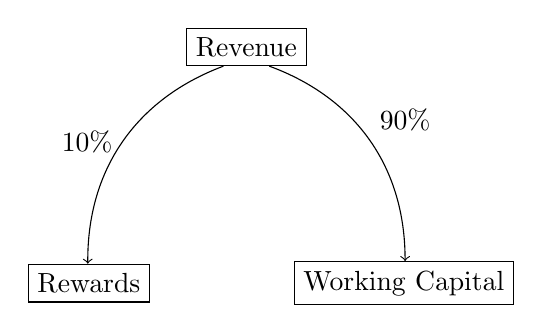
\begin{tikzpicture}
 
 \node[draw] at (-2,-3) (rewards) {Rewards};
 \node[draw] at (2,-3) (workingcapital) {Working Capital};
 \node[draw] at (0,0) (revenue) {Revenue}
    (revenue.-140) edge[bend right=35, ->] node[left]{10{\%}} (rewards)
    (revenue.-40) edge[bend left=35, ->] node[auto]{90{\%}} (workingcapital);
\end{tikzpicture}
\end{center}

\subsection{Claiming Rewards from the reward pot}
Rewards accumulate in the rewards pot. To trigger an actual payout to users (i.e. to make rewards claimable) a special type of proposal is made, proposing that all users should receive a payout based on the reward pot's holdings. 

This reward payout proposal includes the specific currency that should be paid, and only one currency is handled at a time. In the event that the proposal is approved by vote of reputation, then all user's tokens are locked until they claim their payout. Locking is necessary, because the token balance of each account factors into the rewards formula \eqref{eq:reward-claim}. Locking is triggered by incrementing the colony's `most recent payout' counter. 

Our currency contract contains a locking mechanism ensuring that a user cannot move tokens while they have votes to reveal; we use the same mechanism here to ensure that a user cannot move tokens after a payout is approved by the members of the colony but before the user has claimed their rewards. The colony has a counter for each user that is incremented whenever they claim a payout; they can also waive their claim to a payout that will increment this counter.  

While it is of course up to the members of each individual colony to decide, it is advisable that these payout proposals should only be accepted sporadically to keep the gas costs low for the users claiming their payouts, as well as simply to not be a nuisance to the users continually finding their tokens locked.

\textbf{Rewards are only available to accounts that hold both tokens and reputation}, and the amount claimable by each account depends on \emph{both} token balance and reputation (see equation \eqref{eq:reward-claim} below). Therefore we need to have a similar behaviour to `lock' the reputation of the users for the payout. When a payout is activated, the current state of the reputation tree is recorded in the payout itself. Users are paid out according to their reputation in this state, rather than the most recent state, to ensure all users get an appropriate payout and to avoid gaming the system (e.g. ``if I wait until I complete this task, I'll have more reputation and be able to claim more reward'').

\subsubsection*{The Rewards Formula}
The amount that each user ($u_i$) of a colony ($\mathcal{C}$) is entitled to claim ($p_i$) is a function of their colony token holdings ( $t_i$ ) and their total reputation in the colony ($r_i$).

\begin{equation}\label{eq:reward-claim}
 p_i = \frac{\sqrt{t_i r_i}}{\sum\limits_{u_j\in \mathcal{C}} t_j \times \sum\limits_{u_j\in \mathcal{C}} r_j}
\end{equation}

Note that this is very unlikely to payout all the tokens set aside for a payout - the only way it would do so is if everyone had the same proportion of reputation in the colony as they did proportion of tokens in the colony. However, the geometric average is the natural way to capture influence of two variables, and ensures that large token holders must earn large amounts of reputation to get the most from the payouts. The total tokens issued, total reputation and user reputation in the colony are all provable on-chain at claim time via a merkle proof that the \ascode{ReputationRootHash} (Section \ref{sec:reputationmining}) contains some values claimed by the user; the user's balance of colony tokens is trivial to lookup.

After some sufficiently long period of time (500000 blocks), all unclaimed tokens can be reclaimed by the colony and the payout closed. Any users that have not claimed their payout by that point will still have their tokens locked, and they will remain locked until they issue a transaction waiving their claim to the payout (indeed, they already passively did this by not claiming it in a timely fashion). Unclaimed tokens are returned to the reward pot and become part of the next reward cycle.


\subsubsection{Changing the split}\label{subsec:chaning-the-reward-split}

The 10\%/90\% split between rewards and capital can be altered based on a colony-wide vote of tokens and reputation. It requires a majority of both tokens and reputation in order to pass.




\subsection{The Revenue Model of the Colony Network}\label{sec:networkrevenue}
The Colony Network must be able to sustain itself. In particular, the \rc\ (in control of the colony network and reputation mining) maintains the contracts that underpin the network and develops new functionality for the network, the development of which needs to be paid for. Long term, the development and maintenance of the network (including the reputation system) needs to be financed by the network itself. 

\subsubsection{The Network Fee}\label{sec:networkfee}
We propose a fee that is levied on task payments made. When a user claims payment for a task they have done (Section \ref{sec:claiming-bounty}), some small fraction is paid to the network. 

\begin{center}
 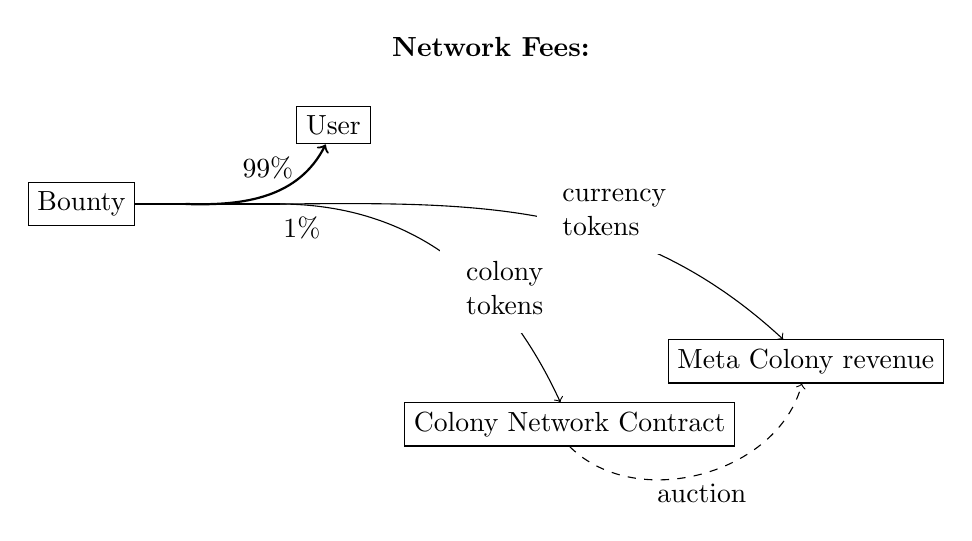
\begin{tikzpicture}
  \node at(0,2) {\textbf{Network Fees:}};
  \node at (-4,0) (dummy) {};
  \node[draw] at (-5.2,0) (bountybox) {Bounty};
  \node at (-2.8,0) (bounty) {}
   (bountybox.east) edge[-, thick] (dummy.east)
   (dummy.east) edge[-] (bounty.east);
   \node at (-2.4,-0.3) {{1\%}};
  \node[draw] at (-2,1) (user) {User};
  \node[draw] at (1,-2.8) (cnc) {Colony Network Contract};
  \node[draw] at (4,-2) (root) {\rc\ revenue}
    (dummy.east) edge[->, bend right=40,out=-25,thick] node[above=2pt] {99{\%}} (user) 
    (dummy.east) edge[->, bend left=30,out=12] node[fill=white,right=10pt] {\begin{tabular}{l} currency \\ tokens\end{tabular}} (root)
    (bounty.east) edge[->, bend left=30,out=35] node[fill=white, below right=-5pt] {\begin{tabular}{l} colony \\ tokens\end{tabular}} (cnc)
    (cnc.south) edge[->, bend right=60, dashed] node[below] {auction} (root)
    ;
 \end{tikzpicture}
\end{center}

The fees thus collected are sent to either the \rc\ (if the payment was in Ether or another whitelisted token) or the Colony Network Contract (if it was in a colony's token).


This idea of a fee is a little unusual for such a decentralised service. One reason why decentralised systems on Ethereum are appealing is that you don't have to pay a fee for the service, other than gas costs. However, we believe that the reputation system will ultimately be appealing enough that a small fee to pay for its existence will be acceptable.

The presence of a fee also means that we have to make some considerations that would be irrelevant to a more traditional decentralised system. For this reason, we will permission the read functions in the \ascode{EternalStorage} contract so that they can only be read by the Colony that owns the \ascode{EternalStorage} contract. This prevents a colony creating a contract that could be used to pay out Ether for tasks without paying the fee based on the status of tasks in the colony.

\subsubsection{The token auction}
The colony tokens collected are auctioned off by the Colony Network Contract, with the auctions denominated in \rcts, the proceeds of which are given to the \rc\ as revenue. These auctions - one for each type of token collected - occur on a regular basis of once a month.

We believe such behaviour would be beneficial for the \rcths\ (whose \rcts\ gain value by having an explicit use) and the \rc\ itself (which turns the fees into \rcts\ which it can then use to fund further development of the network without explicitly buying them back or creating more, diluting existing holders). It also provides an immediate mechanism of price discovery for the colony tokens, which are unlikely to be traded on third-party exchanges until much later in the lifetime of the colony. By auctioning off the collected tokens, we also prevent the \rc\ collecting a large number of different tokens that it has to manage, which would prove cumbersome and annoying for the colony.




\newpage
\section{Allowing more complex behaviour}\label{sec:special-cases}


% \subsection{Example Configurations}\label{sec:example-configs}
The protocol described in this document is concerned with what happens on the Ethereum blockchain. Users of the network however are not expected to ever interact with the contracts manually; instead they will be using front-end applications that make the network's functionality easy to use.

In any colony application we expect a certain amount of \textbf{front-end abstraction} in which complex tools and concepts are presented for the users' convenience, and translated in the background into a sequence of contract interactions on the colony network.

Front-end abstraction lets us realise certain functionality that doesn't \emph{seem} to be part of our protocol by combining the simple elements we have designed in inventive ways. The remainder of this section describes some such cases.

\subsection{Salaried Positions}\label{sec:salary}

The work-for-payment model in the colony network is based around tasks, and on the surface this implies colony-worker relationships that are purely transactional. However the system is flexible enough to accommodate a wider range of employment models. One such example is a \emph{salaried position}.

A salaried position could be realised by creating a special domain representing the position to be filled. The domain could be issued the salary through a priority funding proposal. The employee would be the only person with reputation within that domain and would be able to withdraw funds by creating and self-assigning placeholder tasks that are funded from the domain's pot. A good user interface could hide these implementation details from the users and render salaried positions differently from regular domains.

\subsection{Awarding reputation for work not captured by tasks}

All reputation decays over time, as described in Section \ref{sec:reputation}. This prevents an eternal `reputation aristocracy' and allows reputation to be meaningful even after major changes in the colony token's value. 

Reputation is awarded when a user receives payment of colony tokens --- most commonly as payout from a task, but sometimes from dispute resolution and, in the case of the \rc, from the reputation mining process. We can use the task payout mechanism to award users extra reputation provided there is consensus to do so. 

Consider the scenario in which a founder, or an important early contributor to a colony has almost no reputation left by the time the colony starts earning revenue; perhaps the development of the product took a long time or perhaps the reputation decay rate was sub-optimally high for the particular colony.\footnote{Finding an optimal decay rate for reputation in the network will depend on empirical data collected from early colonies.} Or perhaps the founder was doing a lot of intangible work to get the colony off the ground in the first place and so was never compensated properly through the task system. To get around the limitations of the reputation system and to re-integrate the founder (and make them eligible to receive their rewards), the colony can create a special task that is solely designed to award reputation they are due. To qualify for the payout of tokens (and thereby the reputation), the user in question would have to give the same number of tokens back to the colony. Again, a good frontend abstraction could make such reputation awards easy and intuitive.

The important point is that any limitations imposed by the system can be weakened if there is consensus to do so. The system should not stand in the way of consensus, it should just provide conflict resolution mechanisms for those times in which there is dissent.

\subsection{Objections by non-members}

Having reputation is a prerequisite for creating an objection and triggering the dispute process. Therefore, if an outsider is hired by a colony to perform a task, they will not, on their own, be able to object to the evaluation of their work. However, a good colony frontend may allow them to create the template for an objection, effectively calling for members of the colony to support it and submit the objection to the colony network on-chain on their behalf.  

This is analogous to a member staking only 10\% of the required amount and waiting for further support from their peers (Section \ref{sec:costs-of-disputes}), with the difference being that without any third party support, this `objection' would never be processed on-chain.

\subsection{Proposing an arbitrary transaction by the \ascode{Colony} contract}\label{sec:arbitrary-transaction}
Of course, it is possible that a colony will want to engage in some behaviour that we haven't foreseen, that could be implemented in a contract outside the control of the Colony Network. To that end, we wish to have a mechanism by which a colony can create an arbitrary transaction on the blockchain to interact with contracts and tokens without requiring the network to explicitly support them. As they are powerful, such transactions should be rare occurrences requiring high support thresholds.

Formally, proposing that a colony make an arbitrary transaction on the blockchain is no different from an objection; however the proposal is to change the value of a special variable from zero to the value of the transaction data of the proposed transaction. Such a proposal requires the entire colony to be able to vote (both token holders and reputation holders), as it concerns actions taken `by the contract as a whole'. In the event the proposal is successful, the special variable is set. Another subsequent transaction --- able to be made by anyone --- is able to call a function that executes the transaction in the special variable, and resets it to zero if successful.

\newpage
\section{Conclusion}\label{sec:conclusion}

We have described and defined the Colony Protocol --- an organisational operating system built on Ethereum. It provides a general purpose framework for the creation, management, and operation of decentralised organisations of various kinds.

The specification contained herein represents our current best description of the Colony Protocol. It is however, a working document, and it should be expected that the final specification will differ substantively, both as a consequence of the rapidly changing technological landscape, and the refinement of our understanding of the requirements of decentralised organisation through iterative cycles of development and user testing.
% \newpage
% {Bibliography}
\bibliographystyle{./bibliography/custom.bst}
\bibliography{./bibliography/biblio}
% \begin{thebibliography}{9}
  
\bibitem{The-Nature-of-the-Firm}
  Ronald Coase,
  \emph{The Nature of the Firm\\}
  \verb| http://www3.nccu.edu.tw/~jsfeng/CPEC11.pdf |  
  
  
\bibitem{TruebitWhitepaper}
  Jason Teutsch \& Christian Reitwießner,
  \emph{A scalable verification solution for blockchains\\}
  \verb| people.cs.uchicago.edu/~teutsch/papers/truebit.pdf |
  
\bibitem{ColonyVoting}
  Elena Dimitrova,
  \emph{Token-weighted voting implementation\\}
  \verb| blog.colony.io/token-weighted-voting-implementation-part-1-72f836b5423b |
  
\bibitem{KeynesianBeauty}
  economicsnetwork.ac.uk,
  \emph{References for Keynesian Beauty Contest\\}
  \verb| bit.ly/2pgrvXE |

\bibitem{MerkleTrees}
  Ralph C. Merkle, 1988
  \emph{A digital signature based on a conventional encryption function\\}
  \verb| people.eecs.berkeley.edu/~raluca/cs261-f15/readings/merkle.pdf | 

\bibitem{MerkleInEthereum}
  Vitalik Buterin,
  \emph{Merkling in Ethereum\\}
  \verb| blog.ethereum.org/2015/11/15/merkling-in-ethereum/ |
  
\bibitem{YellowPaper}
  Gavin Wood et el.\\
  The Ethereum ``Yellow Paper'':
  \emph{A secure decentralised generalised transaction ledger\\}
  \verb| ethereum.github.io/yellowpaper/paper.pdf |
  
\bibitem{UpgradingContracts}
  Elena Dimitrova,
  \emph{Writing upgradable contracts in Solidity\\}
  \verb| blog.colony.io/writing-upgradeable-contracts-in-solidity-6743f0eecc88 |
  
\bibitem{erc20}
  Fabian Vogelsteller et al.
  \emph{ERC: Token standard \#20\\}
  \verb| github.com/ethereum/EIPs/issues/20 |
  
\end{thebibliography}

\appendix
\newpage
\section{Gas-efficient reputation penalty in dispute resolution}\label{appendix:rep-transfer}

Once a dispute has been raised and settled one way or the other, the users on the losing side will lose reputation and those on the winning side will gain it. If there is then a disagreement during the reputation mining mechanism, we must be able to calculate on-chain, in a gas-efficient way, a specific reputational consequence of the dispute being settled. All of the reputation changes that each user who was involved in the dispute is only represented by a single entry in the `reputation update log', and so it is necessary to expand upon the process used to do this.

Given that users are able stake small amounts on each objection, an arbitrarily large number of users could theoretically be involved. We must therefore not have any (on-chain) loops in this implementation.

\subsection{Staking}

Let's consider a situation where three users initiate an objection, and two users oppose it with matching funds. In the dispute, the initiating users were found to have been wrong and so will lose their stake.

\begin{table}[h]
\centering
\caption{}
\begin{tabular}{|c|c|c|c|c|c|}
\hline
Stake \# & User  & Staked Amount & $\Sigma^+$ & $\Sigma^-$ \\ \hline
1 & A & 100           & 100                      & 0                                                                       \\ \hline
2 & B & 200           & 300                      & 0                                                                       \\ \hline
3 & C & 300           & 600                      & 0                                                                       \\ \hline
4 & D & -150          & 600                      & -150                                                                    \\ \hline
5 & E & -450          & 600                      & -600                                                                    \\ \hline
\end{tabular}
\end{table}

Let's also assume that all users have the appropriate amount reputation to lose. There are four transfers of reputation that must occur here:

\begin{enumerate}
\item User A loses 100 reputation to User D
\item User B loses 50 reputation to User D
\item User B loses 150 reputation to User E
\item User C loses 300 reputation to User E
\end{enumerate}

Indeed, in a group of $m$ people where some owe the others a debt, the maximum possible of transfers required to make everyone whole is equal to $m-1$. If the reputation being lost has $p$ parents and $c$ children, then there are $2 + 2p + c$ reputation updates that must occur at each of these steps. There are therefore $\left(m-1\right)\times\left(2+2p+c\right)$ reputation updates in total. In the event of a disagreement regarding the reputation state, we must be able to access the $n$th update directly when calculating an update on-chain. This is made possible by additional logging of data when stakes are made.

When a user stakes and opposes some existing stake that does not yet have a counterpart, we record the stakes that it is matching against as well as any remainder.

\begin{table}[ht]
\centering
\caption{}
\begin{tabular}{|c|c|c|c|c|c|}
\hline
Stake & Match From & Match To & Remainder & Tx \# From & Tx \# To\\ \hline
-150  & 1          & 2        & 50      & 1 & 2 \\ \hline
-450  & 2          & 3        & 0       &  3 & 4 \\ \hline
0\tablefootnote{The justification for this line being present is given in section \ref{sec:exactMatching}}  & 0         & 0        & 0 & 5 & 5            \\ \hline
\end{tabular}
\end{table}

When staking, the user supplies the `Match From' and `Match To' arguments. These can be checked to be correct on-chain in constant gas by using the values of $\Sigma^+$ and $\Sigma^-$ recorded alongside previous stakes, and the remainder from the previous match. Then, when a \rcth is asked to prove a particular transaction has been included, they can point to the row in this log that contains that transaction without the contract having to iterate over an arbitrarily long list. The user's client is required to do this iteration locally to find the row, but this does not require any gas expenditure.

\subsection{Exact matching}\label{sec:exactMatching}

For the `reputation update log' to work correctly, we must know exactly how many reputation updates we have to consider. In the above example, it was $4\times (2+2p+c)$, which could be calculated and recorded easily in the update log. However, consider an example where the staked amounts were

\begin{table}[ht]
\centering
\caption{}
\begin{tabular}{|c|c|c|c|c|c|}
\hline
Stake \# & User  & Staked Amount & $\Sigma^+$ & $\Sigma^-$ \\ \hline
1 & A & 100           & 100                      & 0                                                                       \\ \hline
2 & B & 200           & 300                      & 0                                                                       \\ \hline
3 & C & -100           & 300                      & -100                                                                       \\ \hline
4 & D & -200          & 300                      & -300                                                                    \\ \hline
\end{tabular}
\end{table}

Even though there are four people, only two transfers are required --- from user A to user C, and from user B to user D. This is because the users have accidentally matched themselves exactly, and so one transaction makes two users `whole'. In order to accommodate this possibility in the reputation update log, we insert dummy reputation transfers in the log whenever an exact match occurs:

\begin{table}[ht]
\centering
\caption{}
\begin{tabular}{|c|c|c|c|c|c|}
\hline
Stake & Match From & Match To & Remainder & Tx \# From & Tx \# To \\ \hline
-100  & 1          & 1        & 0   & 1 & 1     \\ \hline
 0 & 0          & 0        & 0      & 2 & 2   \\ \hline
-200 & 2          & 2        & 0    & 3 & 3    \\ \hline
 0 & 0          & 0        & 0      & 4 & 4   \\ \hline
\end{tabular}
\end{table}

These dummy insertions occur whenever the remainder is 0 --- i.e. when the new stake has matched only the first unmatched stake (or its remainder) and has done so exactly. This ensures that this log always describes as many transactions as there are people (the last entry is always a dummy transaction as the final transaction will always make two users whole). This means that regardless of how the users have matched up against each other, the event that is recorded in the reputation update log will have a known number of transactions equal to the number of staking users, even if some of those are `null' transactions.

\subsection{Generalisation}

This procedure can also be extended to account for stakes being made in arbitrary orders (i.e. not all of one side followed by all of the other). This can be achieved by making the indices in the `Match From' and `Match To' columns only refer to stakes on one side or the other, and keeping matching lists that map those indices onto the stakes. Altering our first example slightly, we might end up with the stakes in table \ref{appa:modifiedexample} and the log entries in table \ref{appa:modifiedexamplelog}. The list of positive stakes would be [1, 3, 4] and the list of negative stakes would be [2, 5]. The `Match From' and `Match To' indices then refer to the list corresponding to the opposite sign of the stake currently being considered.

\begin{table}[ht]
\centering
\caption{}
\label{appa:modifiedexample}
\begin{tabular}{|c|c|c|c|c|}
\hline
User  & Staked Amount & $\Sigma^+$ & $\Sigma^-$ \\ \hline
A & 100           & 100                      & 0                                                                       \\ \hline
B & -150           & 100                      & -150                                                                     \\ \hline
C & 300           & 400                      & -150                                                                       \\ \hline
D & 200          & 600                      & -150                                                                    \\ \hline
E & -450          & 600                      & -600                                                                    \\ \hline
\end{tabular}
\end{table}

\begin{table}[ht]
\centering
\caption{}
\label{appa:modifiedexamplelog}
\begin{tabular}{|c|c|c|c|c|c|}
\hline
Stake & Match From & Match To & Remainder & Tx \# From & Tx \# To\\ \hline
-150  & 1          & 1        & -50      & 1 & 1 \\ \hline
300   & 1          & 1        & 250      & 2 & 2 \\ \hline
-450  & 2          & 3        & 0       &  3 & 4 \\ \hline
0  & 0         & 0        & 0 & 5 & 5            \\ \hline
\end{tabular}

\end{table}

So for example, in table \ref{appa:modifiedexamplelog}, the stake of -150 is matching against the stake at index 1 in the `positive stake' list which is stake number 1 i.e. the stake from user A. The stake of 300 is matching against the stake at index 1 in the `negative stake' list, which is stake number 2 i.e. (what remains of) the stake from user B.
\newpage
\clearpage
\section{Reputation decay calculation details}\label{appendix:rep-decay}

Reputation in any skill decays by a factor of two every 300000 blocks (roughly every three months). At each update (i.e. after every 300 blocks), the new decayed value ($u_{\rm new}$) is calculated by

$$u_{\rm new} = u_{\rm old} \times \exp\left(-\frac{\ln 2}{1000}\right) = u_{\rm old} \times \exp\left(-k\right).$$


This calculation is applied separately to each user's skill, as well as the number that represents the total of all of those skills in the colony. Due to rounding error with the integer representation on the blockchain, these numbers will drift away from each other. However, we can show the accumulated error will be negligible. The amount of reputation that will be incorrectly missing after the first iteration will be, on average $0.5N$ reputation wei, where $N$ is the number of users that have this skill.\footnote{This ignores the reputation lost by the rounding error on the sum of the users' reputation, but as there is only one total and many more users, this does not change our conclusions. We also note that there is an implicit assumption here that all users have the same amount of reputation; this is a worst-case assumption, as if it is not true then once some users have lost all their reputation the reputation incorrectly lost on each cycle will drop below $0.5N$.} The 0.5 is the average fractional part lost during each calculation.

After the second iteration, the amount of reputation that is incorrectly missing is

$$0.5N\exp\left(-k\right) + 0.5N.$$


The second term here is the incorrectly lost reputation from this second set of calculations. The factor of $\exp\left(-k\right)$ has been introduced to the term representing the incorrectly lost reputation from the first set of calculations because some of that incorrectly lost reputation should have decayed away anyway by this point, and so it shouldn't be considered incorrectly lost.

It is apparent that this is a geometric series, and after $b$ cycles of reputation update have passed, the amount of reputation incorrectly missing ($R_{\rm m}$) is
$$R_{\rm m} = \frac{N}{2} \left(\frac{1-\exp\left(-bk\right)}{1-\exp\left(-k\right)}\right)$$

\noindent where we have used the standard result for the sum of a geometric series. If we started with $R_0$ reputation, then the ratio of the incorrectly missing reputation to the total the colony believes exists is

$$\frac{R_{\rm m}}{R_0\exp\left(-bk\right)}.$$


This ratio becomes 1 when
$$ b = \frac{1}{k}\ln\left(\frac{2R_{\rm 0}}{N}\left(1-\exp\left(-k\right)\right) +1   \right)$$


\noindent which, for conservative values of $R_0 = 200\times10^{18}$ and $N=1000000$ occurs after 38011 iterations, or over 5 years for 15 second blocks. At this point, even though the colony believes some amount of reputation exists, no users have it, and no users can make decisions related to this type of reputation.

This is the end-of-life for an inactive colony; if no activity takes place in it for five years that is worthy of earning reputation, then the colony will be irrecoverable --- no-one will be able to create tasks to earn further reputation. This seems like a reasonable failure mode for an inactive colony, and it would be longer for smaller colonies. 

We now consider the case of an active colony. If the colony is active and creates $A$ new reputation at every update cycle, how does the ratio between the figure taken to be the total reputation and the incorrectly missing reputation change over time?

$R_{\rm m}$ remains the same in this situation, but the total the colony believes exists increases by $A$ each cycle. After $b$ iterations, we can show that the total reputation the colony believes exists is

$$R_{\rm 0}\exp\left(-bk\right) + A\frac{1-\exp\left(-bk\right)}{1-\exp\left(-k\right)}.$$


As $k$ tends to infinity --- which represents the regime of a colony in a steady state --- the ratio between this and $R_{\rm m}$ tends to 
$$\frac{N}{2A}$$

i.e. for the discrepancy to be small between what the colony thinks the total reputation inside it is and the sum of all users' reputations, the reputation earned in each cycle should, on average, be much larger than the number of users. Given that reputation will be expressed in terms of numbers on the order of $10^{18}$, this seems assured.

For calculating the exponential decay, we will use the first-order Taylor expansion of the exponential decay i.e. we approximate $\exp\left(-k\right)$ as $1-k$. Given that $k$ is small, this will be a good approximation --- the second order term is on the order of $10^{-7}$. This error will cause all reputations to decay slightly faster than an exponential, but will not cause the sum of the users' reputation to drift away from the notional sum of the users' reputations in the colony.


\end{document}
